% !TEX program  = lualatex
% !TEX encoding = UTF-8 Unicode
% Kompilieren:  latexmk -lualatex main.tex   (oder: make build)
% ──────────────────────────────────────────────────────────────────────────
\documentclass[a4paper, 12pt, ngerman]{article}

% xcolor wird als Erstes geladen, damit colormeta.tex \definecolor nutzen kann.
\usepackage[table, dvipsnames]{xcolor}

% ── Konfiguration ─────────────────────────────────────────────────────────
%% colormeta.tex — Alle Design-Tokens: Farben, Schriften, Abstände
%% ══════════════════════════════════════════════════════════════════════════
%% NUR DIESE DATEI bearbeiten, um das gesamte Dokument umzugestalten.
%% Keine Farben oder Schriften sind anderswo hart kodiert.
%% ══════════════════════════════════════════════════════════════════════════

%% ── Schriften (werden von fontspec in styles.tex gesetzt) ─────────────────
%% Standard: TeX Gyre-Schriften (immer in TeX Live enthalten, keine
%% Installation erforderlich). Für schönere Alternativen siehe README.md.
\newcommand{\mainfont}{Arial}                % Standard-Schriftart
\newcommand{\sansfont}{Arial}                % Standard-Schriftart
\newcommand{\monofont}{TeX Gyre Cursor}     % Courier-Klon, funktional

%% Optionale Premium-Schriften (Homebrew/manuell installieren):
%% \newcommand{\mainfont}{Source Serif 4}
%% \newcommand{\sansfont}{Source Sans 3}
%% \newcommand{\monofont}{JetBrains Mono}

%% ── Abstände ──────────────────────────────────────────────────────────────
\newcommand{\contentmargin}{2.5cm}   % Seitenrand ringsum
\newcommand{\parskipval}{6pt}        % Abstand zwischen Absätzen
\newcommand{\boxinnersep}{10pt}      % Innenabstand von Info-/Warnboxen

%% ── Farben ────────────────────────────────────────────────────────────────
%% Voraussetzung: xcolor ist bereits mit [table,dvipsnames] in main.tex geladen.

%% Brand / Thema
\definecolor{primary}{HTML}{2E4057}         % Dunkelblau  — Überschriften, Tabellenköpfe
\definecolor{accent}{HTML}{048A81}          % Petrol/Teal — Links, Akzente

%% Infobox (blau-türkis)
\definecolor{infocolor}{HTML}{DDF3F5}       % Hintergrund
\definecolor{infoframe}{HTML}{048A81}       % Rahmen (= accent)

%% Warnbox (amber)
\definecolor{warncolor}{HTML}{FFF4E0}       % Hintergrund
\definecolor{warnframe}{HTML}{E07B39}       % Rahmen

%% Pro / Contra
\definecolor{procolor}{HTML}{D6EDDA}        % Grün-Hintergrund
\definecolor{proframe}{HTML}{1E8A3F}        % Grün-Rahmen
\definecolor{concolor}{HTML}{FADDE1}        % Rot-Hintergrund
\definecolor{conframe}{HTML}{C0392B}        % Rot-Rahmen

%% Codeblock
\definecolor{codeblock}{HTML}{F5F5F5}       % Hintergrund
\definecolor{codeframe}{HTML}{CCCCCC}       % Rahmen

%% Tabellen
\definecolor{tableheader}{HTML}{2E4057}     % Kopfzeilenhintergrund (= primary)
\definecolor{tableheadertext}{HTML}{FFFFFF} % Kopfzeilentext
\definecolor{tablerowalt}{HTML}{EEF2F7}     % Alternierend eingefärbte Zeilen

%% Prozess-Schritte
\definecolor{stepcolor}{HTML}{048A81}       % Schrittnummer-Badge (= accent)

%% Merksatz (Indigo/Lila)
\definecolor{merksatzcolor}{HTML}{F0EEFF}   % Hintergrund
\definecolor{merksatzframe}{HTML}{5C4EC2}   % Rahmen

%% Beispiel (Smaragdgrün)
\definecolor{beispielcolor}{HTML}{E8F5E9}   % Hintergrund
\definecolor{beispielframe}{HTML}{2E9E68}   % Rahmen

%% Aufgabe (Goldgelb)
\definecolor{aufgabecolor}{HTML}{FFF8E1}    % Hintergrund
\definecolor{aufgabeframe}{HTML}{E6A817}    % Rahmen

%% Konzeptkarte
\definecolor{konzeptcolor}{HTML}{F7F9FC}    % Hintergrund (blau-grau)
    % Farben, Schriften, Abstände  ← HIER anpassen
%% usermeta.tex — Persönliche Metadaten
%% Hier Autor, Kurs, Matrikelnummer, Semester und Datum eintragen.
%% ──────────────────────────────────────────────────────────────────────────

\newcommand{\docauthor}{Levin Rüßmann}
\newcommand{\doccourse}{Informatik B.Sc.}
\newcommand{\docstudentid}{838791}
\newcommand{\docsemester}{Sommersemester 2026}
\newcommand{\docdate}{\today}
     % Autor, Kurs, Matrikelnummer, Semester
%% topicmeta.tex — Dokumenten- / Themenmetadaten
%% Hier Titel, Untertitel, Fach und Beschreibung eintragen.
%% ──────────────────────────────────────────────────────────────────────────

\newcommand{\doctitle}{Cloudtechnologie }
\newcommand{\docsubtitle}{Zusammenfassung und Lernzettel}
\newcommand{\docsubject}{Grundlagen der Cloudtechnologie}
\newcommand{\docdescription}{%
  Kompakte Zusammenfassung der Vorlesungsinhalte für die Prüfungsvorbereitung.%
}
    % Titel, Untertitel, Fach, Beschreibung

% ── Pakete & Stile ────────────────────────────────────────────────────────
%% packages.tex — Alle \usepackage-Deklarationen
%% Reihenfolge beachten: xcolor ist bereits in main.tex geladen.
%% Konfiguration (die colormeta-Makros verwendet) erfolgt in styles.tex.
%% ──────────────────────────────────────────────────────────────────────────

%% ── Schriften & Kodierung (LuaLaTeX) ──────────────────────────────────────
\usepackage{fontspec}          % Systemschriften über OpenType/TrueType
\usepackage{unicode-math}      % Unicode-Mathematikschriften

%% ── Sprache ───────────────────────────────────────────────────────────────
\usepackage[ngerman]{babel}
\usepackage{csquotes}          % kontextsensitive Anführungszeichen (für biblatex)

%% ── Seitenlayout ──────────────────────────────────────────────────────────
\usepackage{geometry}          % Seitenränder; konfiguriert in styles.tex
\usepackage{parskip}           % Absatzabstand statt Einzug
\usepackage{setspace}

%% ── Typographie ───────────────────────────────────────────────────────────
\usepackage{microtype}         % optischer Randausgleich, Unterschneidung

%% ── Mathematik ────────────────────────────────────────────────────────────
\usepackage{amsmath}
\usepackage{amssymb}

%% ── Grafiken & Gleitumgebungen ────────────────────────────────────────────
\usepackage{graphicx}
\usepackage{float}
\usepackage{caption}
\usepackage{subcaption}

%% ── Tabellen ──────────────────────────────────────────────────────────────
\usepackage{booktabs}          % professionelle Linien (\toprule, \midrule…)
\usepackage{tabularx}          % auto-breite Spalten (X-Typ)
\usepackage{array}             % erweiterte Spaltentypen
\usepackage{multirow}          % Zellen über mehrere Zeilen
\usepackage{colortbl}          % farbige Tabellenzeilen/-zellen

%% ── Listen ────────────────────────────────────────────────────────────────
\usepackage{enumitem}          % flexible Listen-Konfiguration

%% ── Boxen & Rahmen ────────────────────────────────────────────────────────
\usepackage[most]{tcolorbox}   % bunte Boxen (infobox, warnbox, process…)

%% ── Listings / Code ───────────────────────────────────────────────────────
\usepackage{listings}

%% ── Kopf- & Fußzeile ──────────────────────────────────────────────────────
\usepackage{fancyhdr}

%% ── Überschriften & TOC ───────────────────────────────────────────────────
\usepackage{titlesec}          % Überschriftenformatierung
\usepackage[titles]{tocloft}   % TOC-Formatierung

%% ── Werkzeuge für eigene Befehle ──────────────────────────────────────────
\usepackage{etoolbox}          % \appto, \preto usw. (für procon-Umgebung)
\usepackage{xparse}            % \NewDocumentEnvironment (ggf. im Kernel)
\usepackage{environ}           % \NewEnviron: Body-Kollektion für tabularx-Wrapper

%% ── Bibliographie ─────────────────────────────────────────────────────────
\usepackage[
  backend    = biber,
  style      = authoryear,
  sortlocale = de_DE,
  maxnames   = 3,
  minnames   = 1,
]{biblatex}
\addbibresource{bibliography/sources.bib}

%% ── Hyperlinks (muss fast zuletzt geladen werden) ─────────────────────────
\usepackage{hyperref}          % konfiguriert in styles.tex via \hypersetup
\usepackage{bookmark}

%% ── Diverses ──────────────────────────────────────────────────────────────
\usepackage{lipsum}            % Blindtext für Beispiele
   % alle \usepackage-Deklarationen
%% commands.tex — Eigene Umgebungen und Befehle
%% Alle Farben kommen aus config/colormeta.tex; nichts ist hart kodiert.
%% ──────────────────────────────────────────────────────────────────────────

%% ══════════════════════════════════════════════════════════════════════════
%% 1.  process  +  \step{text}
%%     Nummerierter Schritt-für-Schritt-Ablauf mit farbigem linken Rand.
%%
%%  Verwendung:
%%    \begin{process}
%%      \step{Erster Schritt}
%%      \step{Zweiter Schritt}
%%    \end{process}
%% ══════════════════════════════════════════════════════════════════════════
\newcounter{procstep}

\newenvironment{process}{%
  \setcounter{procstep}{0}%
  \begin{tcolorbox}[
    enhanced,
    breakable,
    boxrule         = 0pt,
    frame hidden,
    borderline west = {3pt}{0pt}{stepcolor},
    colback         = stepcolor!6!white,
    left            = 10pt,
    right           = 8pt,
    top             = 6pt,
    bottom          = 6pt,
    arc             = 3pt,
  ]%
}{%
  \end{tcolorbox}%
}

\newcommand{\step}[1]{%
  \stepcounter{procstep}%
  \vspace{4pt}%
  \noindent
  \colorbox{stepcolor}{%
    \color{white}\bfseries\small\hspace{3pt}\theprocstep\hspace{3pt}%
  }%
  \hspace{6pt}#1\par
}

%% ══════════════════════════════════════════════════════════════════════════
%% 2.  infobox[Titel]
%%     Farbige Infobox mit optionalem fettem Titel.
%%
%%  Verwendung:
%%    \begin{infobox}[Mein Titel] ... \end{infobox}
%%    \begin{infobox}             ... \end{infobox}   % ohne Titel
%% ══════════════════════════════════════════════════════════════════════════
\NewDocumentEnvironment{infobox}{O{}}{%
  \def\lzinfoboxtitle{#1}%
  \ifdefempty{\lzinfoboxtitle}{%
    %% ── Ohne Titel ──
    \begin{tcolorbox}[
      enhanced, breakable,
      colback  = infocolor,
      colframe = infoframe,
      boxrule  = 1pt,
      arc      = 4pt,
      left     = \boxinnersep,
      right    = \boxinnersep,
      top      = \boxinnersep,
      bottom   = \boxinnersep,
    ]%
  }{%
    %% ── Mit Titel ──
    \begin{tcolorbox}[
      enhanced, breakable,
      colback      = infocolor,
      colframe     = infoframe,
      boxrule      = 1pt,
      arc          = 4pt,
      left         = \boxinnersep,
      right        = \boxinnersep,
      top          = \boxinnersep,
      bottom       = \boxinnersep,
      title        = {\textbf{\lzinfoboxtitle}},
      fonttitle    = \bfseries\color{white},
      colbacktitle = infoframe,
      attach boxed title to top left = {yshift=-2mm, xshift=4mm},
      boxed title style = {
        colback  = infoframe,
        colframe = infoframe,
        arc = 3pt, top = 2pt, bottom = 2pt,
      },
    ]%
  }%
}{%
  \end{tcolorbox}%
}

%% ══════════════════════════════════════════════════════════════════════════
%% 3.  warnbox[Titel]
%%     Warnbox / Tipp-Box mit optionalem fettem Titel.
%% ══════════════════════════════════════════════════════════════════════════
\NewDocumentEnvironment{warnbox}{O{}}{%
  \def\lzwarnboxtitle{#1}%
  \ifdefempty{\lzwarnboxtitle}{%
    %% ── Ohne Titel ──
    \begin{tcolorbox}[
      enhanced, breakable,
      colback  = warncolor,
      colframe = warnframe,
      boxrule  = 1pt,
      arc      = 4pt,
      left     = \boxinnersep,
      right    = \boxinnersep,
      top      = \boxinnersep,
      bottom   = \boxinnersep,
    ]%
  }{%
    %% ── Mit Titel ──
    \begin{tcolorbox}[
      enhanced, breakable,
      colback      = warncolor,
      colframe     = warnframe,
      boxrule      = 1pt,
      arc          = 4pt,
      left         = \boxinnersep,
      right        = \boxinnersep,
      top          = \boxinnersep,
      bottom       = \boxinnersep,
      title        = {\textbf{\lzwarnboxtitle}},
      fonttitle    = \bfseries\color{white},
      colbacktitle = warnframe,
      attach boxed title to top left = {yshift=-2mm, xshift=4mm},
      boxed title style = {
        colback  = warnframe,
        colframe = warnframe,
        arc = 3pt, top = 2pt, bottom = 2pt,
      },
    ]%
  }%
}{%
  \end{tcolorbox}%
}

%% ══════════════════════════════════════════════════════════════════════════
%% 4.  procon  +  \pro{text}  \con{text}
%%     Zwei-Spalten-Gegenüberstellung Vorteile / Nachteile.
%%     Alle \pro{} und \con{} werden gesammelt und am Ende nebeneinander
%%     als zwei tcolorbox-Minipages gesetzt.
%%
%%  Verwendung:
%%    \begin{procon}
%%      \pro{Vorteil 1}
%%      \con{Nachteil 1}
%%    \end{procon}
%% ══════════════════════════════════════════════════════════════════════════
\newenvironment{procon}{%
  \def\lzproitems{}%
  \def\lzconitems{}%
  % \def statt \newcommand: kein Fehler beim mehrfachen Aufruf
  % ##1 = #1 auf zweiter Makro-Ebene innerhalb von \newenvironment
  \def\pro##1{\appto\lzproitems{\item ##1}}%
  \def\con##1{\appto\lzconitems{\item ##1}}%
}{%
  \par\smallskip\noindent
  \begin{minipage}[t]{0.475\linewidth}
    \begin{tcolorbox}[
      enhanced,
      colback      = procolor,
      colframe     = proframe,
      boxrule      = 1pt,
      arc          = 4pt,
      title        = {Vorteile},
      fonttitle    = \bfseries\color{white},
      colbacktitle = proframe,
      left = 6pt, right = 6pt, top = 4pt, bottom = 4pt,
    ]
      \begin{itemize}[leftmargin=*, nosep, topsep=0pt]
        \lzproitems
      \end{itemize}
    \end{tcolorbox}
  \end{minipage}%
  \hfill
  \begin{minipage}[t]{0.475\linewidth}
    \begin{tcolorbox}[
      enhanced,
      colback      = concolor,
      colframe     = conframe,
      boxrule      = 1pt,
      arc          = 4pt,
      title        = {Nachteile},
      fonttitle    = \bfseries\color{white},
      colbacktitle = conframe,
      left = 6pt, right = 6pt, top = 4pt, bottom = 4pt,
    ]
      \begin{itemize}[leftmargin=*, nosep, topsep=0pt]
        \lzconitems
      \end{itemize}
    \end{tcolorbox}
  \end{minipage}%
  \par\smallskip
}

%% ══════════════════════════════════════════════════════════════════════════
%% 5.  codebox
%%     Monospace-Block mit grauem Hintergrund (für kurze Ausschnitte).
%%     Für Syntax-Highlighting: listings-Paket nutzen (siehe packages.tex).
%% ══════════════════════════════════════════════════════════════════════════
\newenvironment{codebox}{%
  \begin{tcolorbox}[
    enhanced,
    breakable,
    colback  = codeblock,
    colframe = codeframe,
    boxrule  = 0.5pt,
    arc      = 3pt,
    left     = 8pt,
    right    = 8pt,
    top      = 6pt,
    bottom   = 6pt,
    fontupper = \ttfamily\small,
  ]%
}{%
  \end{tcolorbox}%
}

%% ══════════════════════════════════════════════════════════════════════════
%% 6.  \sidetables{Inhalt links}{Inhalt rechts}
%%     Zwei beliebige Inhalte (z. B. Tabellen, Listen) nebeneinander.
%% ══════════════════════════════════════════════════════════════════════════
\newcommand{\sidetables}[2]{%
  \par\smallskip\noindent
  \begin{minipage}[t]{0.475\linewidth}
    #1
  \end{minipage}%
  \hfill
  \begin{minipage}[t]{0.475\linewidth}
    #2
  \end{minipage}%
  \par\smallskip
}

%% ══════════════════════════════════════════════════════════════════════════
%% 7.  stdtable{Spaltendefinition}{Kopfzeile}
%%     Formatierte Tabelle mit farbiger Kopfzeile und alternierenden Zeilen.
%%     Spaltentypen: l r c  für Text; X für auto-breite Spalten; p{…} für
%%     feste Breite. X-Spalten sind durch tabularx möglich, weil \NewEnviron
%%     (environ-Paket) den Body komplett sammelt, bevor tabularx ihn scannt.
%%
%%  Verwendung:
%%    \begin{stdtable}{l X X}{Algorithmus & Kompl. & Notiz}
%%      Bubble Sort & $O(n^2)$ & Einfach \\
%%    \end{stdtable}
%% ══════════════════════════════════════════════════════════════════════════
\NewEnviron{stdtable}[2]{%
  \par\smallskip
  \rowcolors{2}{tablerowalt}{white}%
  \begin{center}%
  \begin{tabularx}{\linewidth}{#1}%
  \rowcolor{tableheader}%
  \color{tableheadertext}\bfseries #2\\[\jot]%
  \BODY
  \end{tabularx}%
  \end{center}%
  \rowcolors{1}{}{}%   Reset: verhindert Übertrag auf nachfolgende Tabellen
  \par\smallskip
}
   % eigene Umgebungen und Befehle
%% styles.tex — Schriften, Seitenlayout, Kopf-/Fußzeile, TOC, Hyperlinks
%% Alle Farben und Schriften kommen aus config/colormeta.tex.
%% ──────────────────────────────────────────────────────────────────────────

%% ── Schriften (fontspec) ──────────────────────────────────────────────────
\setmainfont{\mainfont}[
  Ligatures = TeX,
]
\setsansfont{\sansfont}[
  Ligatures = TeX,
]
\setmonofont{\monofont}[
  Scale = 0.88,
]

%% ── Seitenlayout (geometry) ───────────────────────────────────────────────
\geometry{
  a4paper,
  top    = \contentmargin,
  bottom = \contentmargin,
  left   = \contentmargin,
  right  = \contentmargin,
  headheight = 15pt,
}

%% ── Absatzformat ─────────────────────────────────────────────────────────
\setlength{\parskip}{\parskipval}
\setlength{\parindent}{0pt}

%% ── Grafikpfad ───────────────────────────────────────────────────────────
\graphicspath{{assets/images/}}

%% ── Überschriften (titlesec) ─────────────────────────────────────────────
\AddToHook{cmd/section/before}{\clearpage}

\titleformat{\section}
  {\Large\bfseries\color{primary}}         % Format
  {\color{primary}\thesection}             % Label
  {0.75em}                                  % Abstand Label–Text
  {}                                        % Vor dem Titel
  [\color{primary!50!white}\rule{\linewidth}{0.6pt}]  % Unter dem Titel

\titleformat{\subsection}
  {\large\bfseries\color{primary!80!black}}
  {\color{accent}\thesubsection}
  {0.75em}
  {}

\titleformat{\subsubsection}
  {\normalsize\bfseries\color{accent}}
  {\thesubsubsection}
  {0.75em}
  {}

\titlespacing*{\section}      {0pt}{1.4ex plus .4ex minus .2ex}{0.6ex}
\titlespacing*{\subsection}   {0pt}{1.2ex plus .3ex minus .2ex}{0.4ex}
\titlespacing*{\subsubsection}{0pt}{1.0ex plus .2ex minus .1ex}{0.3ex}

%% ── Inhaltsverzeichnis (tocloft) ─────────────────────────────────────────
\renewcommand{\cftsecfont}{\bfseries\color{primary}}
\renewcommand{\cftsecpagefont}{\bfseries\color{primary}}
\renewcommand{\cftsubsecfont}{\color{primary!80!black}}
\renewcommand{\cftsubsecpagefont}{\color{primary!80!black}}
\setlength{\cftsecindent}{0pt}
\setlength{\cftsubsecindent}{1.5em}
\setlength{\cftbeforesecskip}{2pt}

%% ── Kopf- und Fußzeile (fancyhdr) ────────────────────────────────────────
\pagestyle{fancy}
\fancyhf{}
\fancyhead[L]{\small\color{primary}\docsubject}
\fancyhead[R]{\small\color{primary}\docauthor}
\fancyfoot[C]{\small\thepage}
\renewcommand{\headrulewidth}{0.4pt}
\renewcommand{\footrulewidth}{0pt}
% Auch Kapitelanfangsseiten mit fancyhdr versehen
\fancypagestyle{plain}{%
  \fancyhf{}%
  \fancyfoot[C]{\small\thepage}%
  \renewcommand{\headrulewidth}{0pt}%
}

%% ── Hyperlinks (hyperref) ────────────────────────────────────────────────
\hypersetup{
  colorlinks = true,
  linkcolor  = primary,
  urlcolor   = accent,
  citecolor  = accent,
  pdftitle   = {\doctitle},
  pdfauthor  = {\docauthor},
  pdfsubject = {\docsubject},
}

%% ── Captions ─────────────────────────────────────────────────────────────
\captionsetup{
  font       = small,
  labelfont  = {bf, color=primary},
  labelsep   = period,
}

%% ── Titelseite (wird in main.tex mit \makelernzetteltitle aufgerufen) ─────
\newcommand{\makelernzetteltitle}{%
  \begin{titlepage}
    \centering
    \vspace*{2.5cm}

    % Fach-Badge
    {\sffamily\small\color{white}%
      \colorbox{accent}{\hspace{6pt}\docsubject\hspace{6pt}}%
    }\par
    \vspace{1.2cm}

    % Haupttitel
    {\Huge\bfseries\color{primary}\doctitle\par}
    \vspace{0.5cm}
    {\large\color{accent}\docsubtitle\par}

    \vspace{0.8cm}
    % Trennlinie
    {\color{primary!40!white}\rule{0.6\linewidth}{1.5pt}}\par
    \vspace{0.5cm}

    % Beschreibung
    {\normalsize\color{primary!70!black}\docdescription\par}

    \vfill

    % Metadaten-Tabelle
    \begin{tabular}{@{}r@{\hspace{8pt}}l@{}}
      \color{primary!60!black}\small Autor            & \docauthor      \\[2pt]
      \color{primary!60!black}\small Matrikelnummer   & \docstudentid   \\[2pt]
      \color{primary!60!black}\small Studiengang      & \doccourse      \\[2pt]
      \color{primary!60!black}\small Semester         & \docsemester    \\[2pt]
      \color{primary!60!black}\small Datum            & \docdate        \\
    \end{tabular}

    \vspace{2cm}
    % Fußleiste
    {\color{primary!30!white}\rule{\linewidth}{0.6pt}}\par
    \vspace{0.3cm}
    {\small\color{primary!50!black}\sffamily Lernzettel}
  \end{titlepage}%
  \clearpage
}
     % Schriften, Seitenlayout, Kopf-/Fußzeile, TOC

% ──────────────────────────────────────────────────────────────────────────
\begin{document}

% Titelseite (generiert aus usermeta + topicmeta)
\makelernzetteltitle

% Inhaltsverzeichnis
\tableofcontents
\clearpage

% ── Inhalt ────────────────────────────────────────────────────────────────
% Block 1 – Grundlagen: Was ist Cloud?
\section{Grundbegriffe}
\subsection{Cloud}
Eine \textbf{Cloud} bezeichnet das Auslagern von Rechenaufgaben und Speicher auf
entfernte Computer, die nicht der eigene, lokale Rechner sind. Eine Cloud kann
unterschiedliche Aufgaben übernehmen; meistens sind es \textbf{Compute} (Rechenleistung)
und \textbf{Storage} (Speicher).
\subsection{Compute}
% LEKTORAT (Redundanz): Compute wird hier kanonisch erklärt. Die zuvor
% doppelte Compute-Erklärung in cloud_services.tex wurde entfernt.
\textbf{Compute} bedeutet im Cloud-Kontext, dass eine Cloud Rechenleistung
bereitstellt. Das kann auf vielfältige Weise geschehen: von einfachen
virtuellen Maschinen (VMs) über \textit{Managed Services} zum Hosten eigener
Anwendungen bis hin zu SaaS-Produkten wie \textit{Microsoft~365}.
\begin{figure}[H]
    \centering
    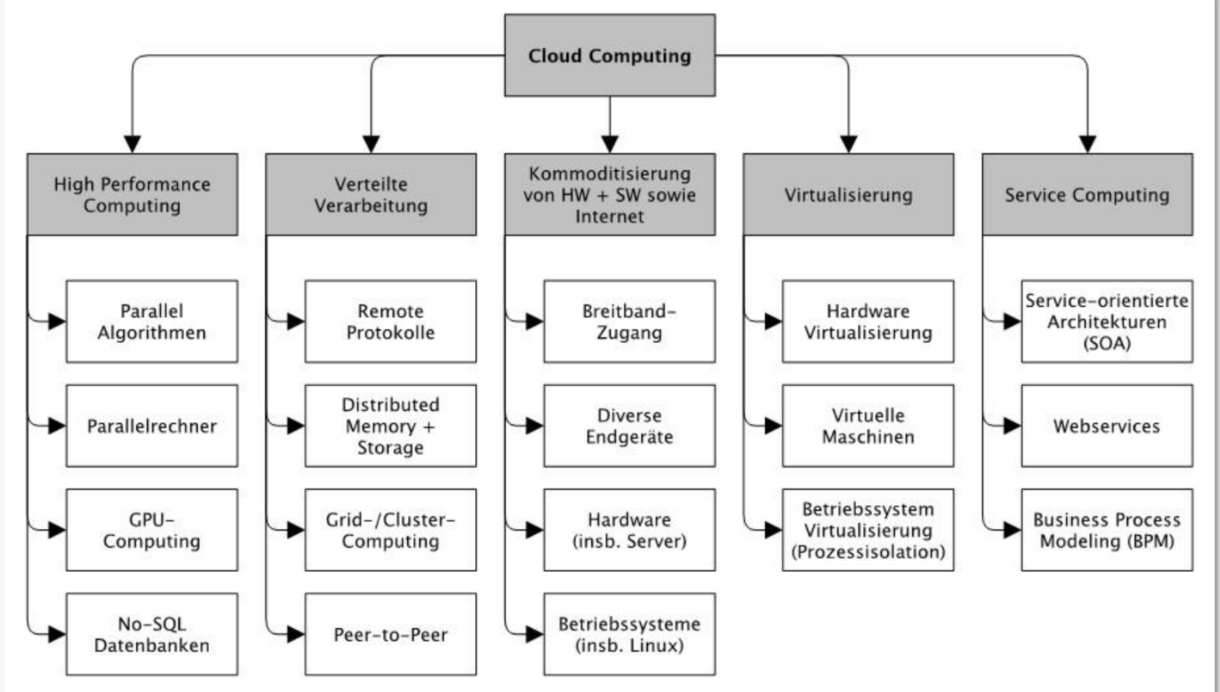
\includegraphics[width=\textwidth]{assets/images/CloudComputingErklaert}
    \caption{Cloud Computing erklärt}
\end{figure}
\subsection{Storage}
\textbf{Storage} bedeutet im Cloud-Kontext die Bereitstellung von Speicher. Auch das
kann auf unterschiedlichste Weise geschehen: als einfacher Cloud-Speicher
ähnlich einer Festplatte, als Speicher für Webanwendungen (etwa um Nutzerdaten
abzulegen) oder als Speicher, der in SaaS-Produkte wie \textit{Microsoft~365} oder
Streaming-Dienste wie \textit{Netflix} integriert ist.
          % Cloud, Compute, Storage
\section{Virtualisierung}
\textbf{Virtualisierung} ist ein schon lange bestehendes Konzept. Dabei wird auf einem
physischen Computer per Software eine andere, \emph{isolierte Umgebung} abstrahiert.
Bekannt ist das Konzept beispielsweise durch \textit{Oracle VirtualBox}. Als Abstraktion
von Hardware-Ressourcen durch Software ist Virtualisierung zugleich der
\emph{Grundstein} für Cloud-Technologie: Erst sie ermöglicht \textit{Resource Pooling}, denn
sonst könnten keine voneinander getrennten Umgebungen auf einem Server
existieren.
\subsection{Wie nutzt eine Cloud Virtualisierung?}
\subsubsection{Virtuelle Maschinen (Virtual Machine)}
Bei einer \textbf{VM} (kurz für Virtuelle Maschine) wird eine \emph{eigenständige, isolierte}
Instanz auf einem physischen System abstrahiert. Dadurch kann man
beispielsweise auf einem Windows-PC ein Linux-Betriebssystem innerhalb einer VM
ausführen. In der Cloud wird dies für \textit{Resource Pooling} genutzt, also das
Aufteilen eines physischen Servers in mehrere kleinere, unabhängige Instanzen.
So werden \textit{Infrastructure as a Service (IaaS)} und dynamische Skalierung erst
ermöglicht.
\subsubsection{Virtuelles Netzwerk}
Ein \textbf{virtuelles Netzwerk} ermöglicht die Kommunikation zwischen VMs sowie mit
externen Systemen. Durch \textit{Peering} – das direkte Verbinden zweier virtueller
Netzwerke – können Services untereinander kommunizieren, ohne den Umweg über
das öffentliche Internet nehmen zu müssen. Über \textit{VPNs} (Virtual Private Network)
lässt sich zudem eine verschlüsselte Direktverbindung zu
\textit{On-Premises}-Rechenzentren herstellen, um sicher mit Cloud-Services zu
kommunizieren.
\subsubsection{Speichervirtualisierung}
Bei der \textbf{Speichervirtualisierung} werden mehrere physische Speichermedien per
Software zu einem einzigen logischen Speicherpool zusammengefasst und
abstrahiert. Das ermöglicht beispielsweise Dienste wie \textit{Google Drive} und \textit{iCloud}
oder – im Enterprise-Kontext – \textit{Azure Managed Disks}.

\subsubsection{Hypervisor}
Ein \textbf{Hypervisor} ist die Software, die Arbeitsspeicher, Rechenleistung und
Speicher in Pools zusammenfasst. Dadurch lassen sich auf einer physischen
Maschine viele VMs erstellen. Der Hypervisor stellt den einzelnen virtuellen
Maschinen die zugewiesenen Ressourcen bereit und verwaltet deren Planung im
Verhältnis zu den physischen Ressourcen. Die Ausführung übernimmt nach wie vor
\emph{die physische Hardware}: Die CPU führt weiterhin die CPU-Befehle aus, wie sie
etwa von den VMs angefordert werden, während der Hypervisor die Planung
übernimmt.

\begin{table}[h]
    \centering
    \begin{tabular}{|l|p{5cm}|p{5cm}|}
        \hline
        \textbf{Merkmal} & \textbf{Typ 1 (Bare-Metal)} & \textbf{Typ 2 (Gehostet)} \\
        \hline
        Ausführung & Direkt auf der Hardware & Auf einem Host-Betriebssystem \\
        \hline
        Host-OS & Keins, ersetzt das OS & Benötigt ein Host-OS \\
        \hline
        Ressourcenzuweisung & Direkt durch den Hypervisor & Über das Host-OS \\
        \hline
        Beispiele & \textit{VMware ESXi}, \textit{KVM} & \textit{Oracle VirtualBox}, \textit{VMware Workstation} \\
        \hline
    \end{tabular}
    \caption{Vergleich Hypervisor Typ~1 und Typ~2}
    \label{tab:hypervisor}
\end{table}


    % technischer Grundstein (ermöglicht Resource Pooling)
\section{Cloud nach NIST}
Die NIST definiert Cloud nicht über Marketingbegriffe, sondern über 5 technische und organisatorische Eigenschaften.
\subsection{NIST – National Institute of Standards and Technology}
NIST ist eine US-amerikanische Behörde. Die NIST ist gleichzeitig eine Großforschungseinrichtung mit den Forschungsbereichen Messtechnik von physikalisch-technischen Konstanten und heutzutage auch Informationssicherheit.
\subsection{On-Demand Self-Service}
Ein Cloud Nutzer kann eigenständig Services erwerben. Ohne IT-Abteilung, Callcenter oder Vermittler. Auf einer Cloud sollte man jederzeit zugreifen können sowie die Cloud jederzeit kündigen können. Zusätzlich läuft die Cloud über automatisierte Schnittstellen.
\subsection{Broad Network Access}
Eine Cloud sollte von überall mit internetfähigem Gerät erreichbar sein. Da der Cloud-Service flächendeckend verfügbar ist.
\subsection{Resource Pooling}
Bei einer Cloud werden Ressourcen geteilt. Das bedeutet mehrere Nutzer teilen sich die Rechenleistung eines Servers. Um Datenschutz der jeweiligen Region oder Zone zu gewährleisten muss der Cloud Provider entsprechende Maßnahmen treffen.
\subsection{Rapid Elasticity}
Elastizität im Cloud Kontext bedeutet das eine Anwendung automatisch skaliert werden kann, also das ein richtiges Ressourcenlevel aus Rechenleistung, Speicher, Bandbreite und Speicher variabel gewählt wird. Dies ist wichtig um möglichst gut auf Nutzung reagieren zu können ohne das ein Ausfall passiert. Ein beliebtes Beispiel ist hier der Online Shop an Black Friday.
\subsection{Measured Service}
Ein Service in der Cloud sollte messbar sein. Das ist gerade wichtig für Pay-as-you-go, also das man nur das zahlt was man auch wirklich nutzt. Dadurch ist eine höhere Transparenz möglich, wodurch man Kosten besser kalkulieren kann.
        % formale NIST-Definition (5 Eigenschaften)
\section{Cloud Begriffe}
\subsection{Cloud consumer}
Ein Cloud Consumer ist der Nutzer von durch eine Cloud bereitgestellten Diensten. Dieser entscheidet über seine eigenen Abonnements. Ein Beispiel ist wenn man sich für ein Claude – Also den KI Chatbot – Abo entscheidet ist man ein Cloud Consumer. Dasselbe gilt für iCloud, Spotify, Apple Music und Netflix. Im Enterprise Kontext ist das noch mal anders dort sind typische Abonnements Microsoft 365, Salesforce oder auch Abonnements bei Cloud Providern wie bei Azure.
\subsection{Cloud Provider}
Ein Cloud Provider stellt die Infrastruktur und die Services einer Cloud bereit. Abseits davon sind die Provider für Betrieb und Sicherheit der Dienste verantwortlich. Beispiele sind die Hyperscaler wie Azure, AWS und Google aber auch europäische Anbieter wie beispielsweise Hetzner sind Cloud Provider.
\subsection{Cloudauditor}
Ein Cloud Auditor prüft Rechenzentren von Cloud Providern und ob diese sich an den Datenschutz und Compliance halten.
\subsection{Cloud broker}
Ein Cloud Broker ist ein unabhängiger Anbieter der zwischen Cloud Consumer und Provider kommuniziert. Ein Beispiel wäre ein Systemhaus das Lizenzen einer Cloud kauft und Consumer diese samt Support und Konfiguration weiter verkauft.
\subsection{Cloud carrier}
Ein Cloud Carrier ist für eine sichere und stabile Datenübertragung von Cloud Consumer zu Cloud Provider verantwortlich.
         % Akteure: Consumer, Provider, Auditor …

% Block 2 – Cloud-Eigenschaften
\section{Cloud-Eigenschaften}
\subsection{Skalierung – Scalability}
Skalierung im Cloud Kontext bedeutet Rechenleistung, Speicher und Netzwerkbandbreite dynamisch an sich ändernde Workloads anzupassen. Es wird in zwei Arten unterteilt.
\subsubsection{Horizontale Skalierung}
Bei horizontaler Skalierung wird ein Workload auf mehreren Servern ausgeführt bzw ausgeweitet.
\subsubsection{Vertikale Skalierung}
Ein bestehender Server wird aufgerüstet durch beispielsweise mehr RAM.
\subsection{Elastizität – Elasticity}
Elastizität im Cloud Kontext bedeutet das eine Anwendung automatisch skaliert werden kann.
\subsection{Hochverfügbarkeit – Availability}
Hochverfügbarkeit bedeutet das eine in der Cloud gehostete Anwendung immer erreichbar ist. Wie viele Ausfälle im Jahr prozentual passieren dürfen ist in einem SLA (Service Level Agreement) festgehalten.
\subsubsection{SLA – Service Level Agreement}
In einem SLA ist Uptime, meist als Nines also z.B. 5 Nines --> 99,999, Reaktion und Lösungszeit, Leistungsparameter, Ausstiegsstrategien und Datenportabilität sowie Sicherheit und Compliance geregelt.
    % Skalierung, Elastizität, Hochverfügbarkeit/SLA

% Block 3 – Infrastruktur: Wo läuft Cloud?
\section{Regionen und Verfügbarkeitszonen}
\subsection{Region}
Eine Cloud-Region ist ein geografischer Bereich, der aus mehreren
Verfügbarkeitszonen besteht. Regionen sind meist nach Himmelsrichtung
oder Lage benannt, zum Beispiel \textit{Deutschland West Central} oder
\textit{North Europe} bei Azure. Die Wahl der Region bestimmt, wo Daten
physisch gespeichert werden (Datenresidenz) und beeinflusst die Latenz
zu den Endnutzern. Jede Region ist physisch und logisch von anderen
Regionen isoliert, sodass ein Ausfall einer Region andere nicht
beeinträchtigt.
\subsection{Verfügbarkeitszonen}
Eine Verfügbarkeitszone (engl. \textit{Availability Zone}) ist eine
physisch getrennte Einheit innerhalb einer Region. Sie besteht aus einem
oder mehreren Rechenzentren mit eigener Stromversorgung, Kühlung und
Netzwerkanbindung. Verfügbarkeitszonen innerhalb einer Region sind über
redundante Hochgeschwindigkeitsverbindungen mit geringer Latenz
verbunden. Durch die Verteilung von Diensten auf mehrere Zonen können
Anwendungen auch bei einem Zonenausfall verfügbar bleiben
(Hochverfügbarkeit).
     % Region & Verfügbarkeitszonen
\section{Rechenzentrum}
Moderne Rechenzentren haben viel Anforderung die sie Erfüllen müssen. 
\begin{figure}[H]
    \centering
    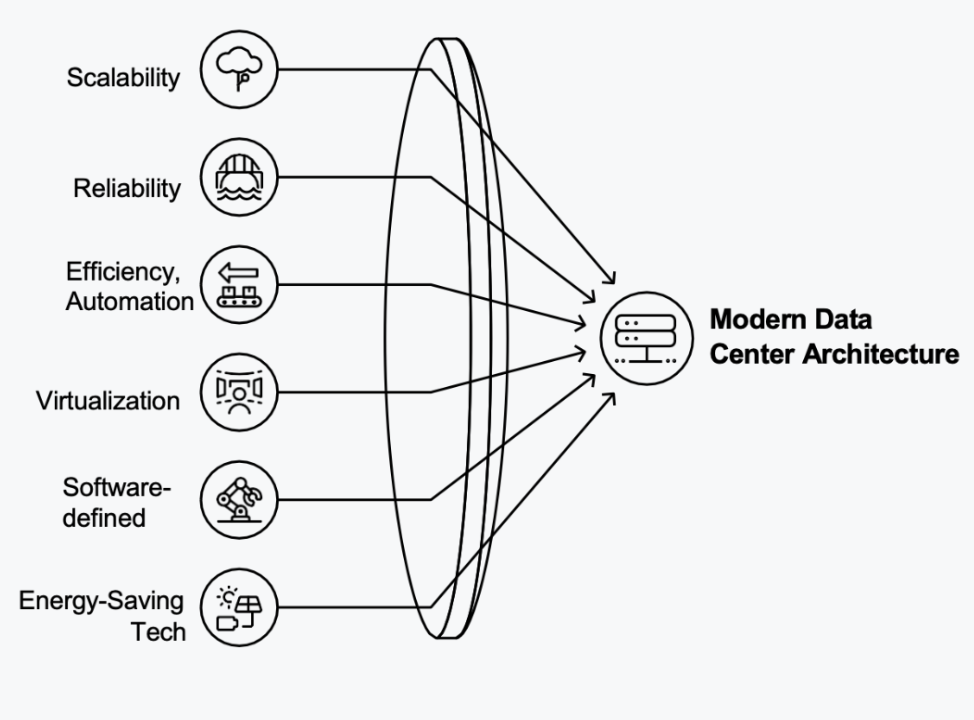
\includegraphics[width=\textwidth]{assets/images/DatacenteArchteiktur}
    \caption{Archietekutr eines Rechenzentrum}
\end{figure}
\subsection{Kompoenten eines Rechenzentrum}
\begin{itemize}
  \item Netzteile (PDU)
  \item Kühl Systeme
  \item Server
  \item Managment Software und Automation
  \item Physische Sicherheits Vorkehrung
  \item Netzwerk Eqiument
  \item Speicher Systeme
\end{itemize}
\subsection{Aufrecht erhaltung eine Rechenzentrum}
\begin{figure}[H]
  \centering
  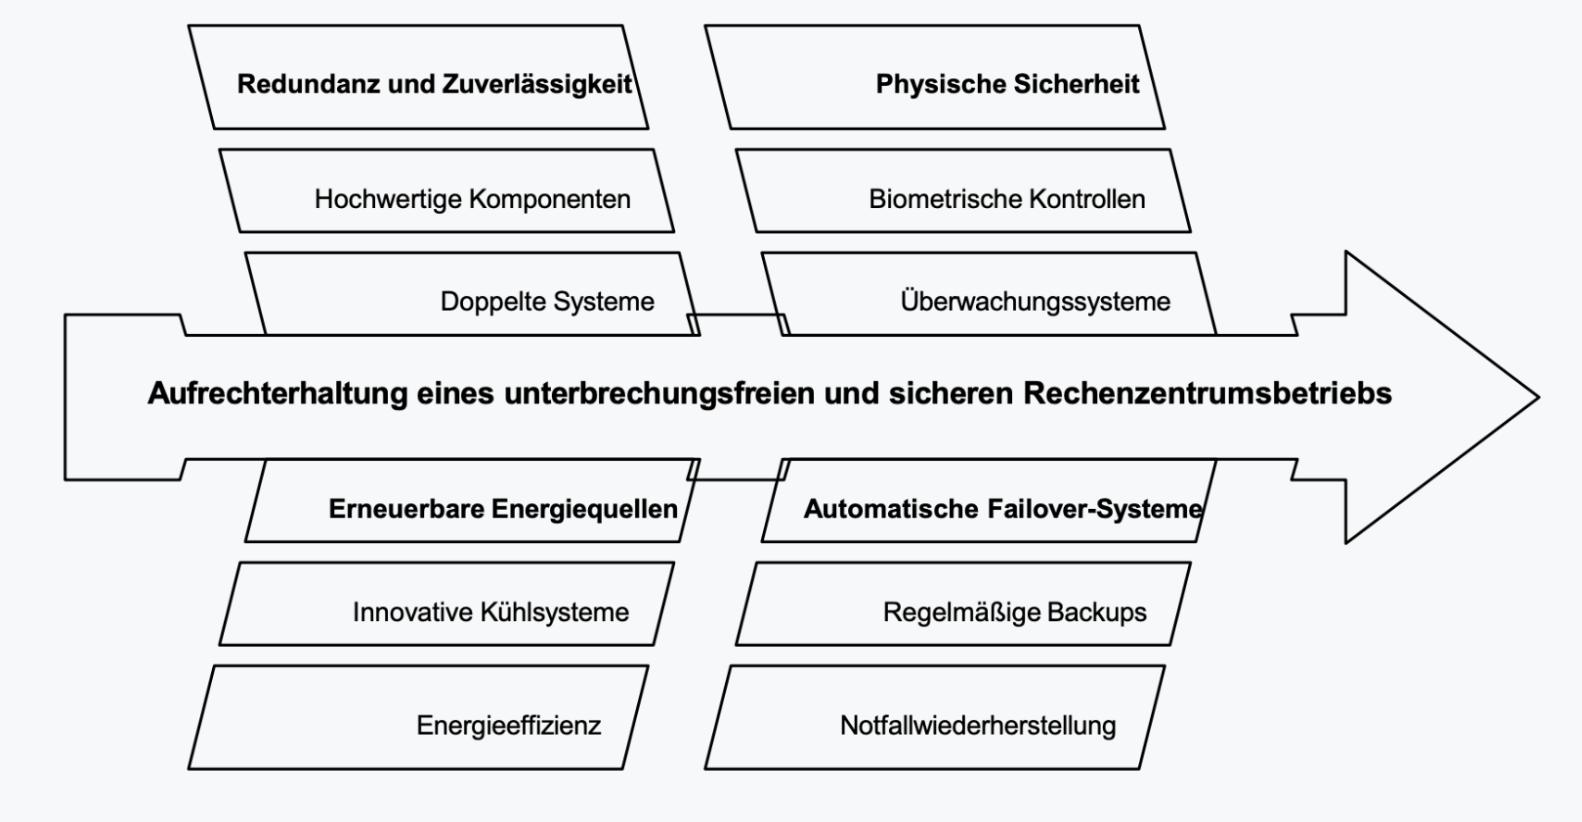
\includegraphics[width=\textwidth]{assets/images/AufrechtErhaltungRechenzetrum}
  \caption{Aufrechterhaltung eines unterbrechungsfreien und sicheren Rechenzentrumsbetriebs}
\end{figure}
\section{Internet Service Provider – ISP}
Ein ISP bezeichnet ein Unternehmen, das Endkunden und Organisationen den Zugang
zum Internet sowie damit verbundene Dienste wie Webhosting,
Domain-Registrierung und E-Mail-Hosting ermöglicht.
\begin{figure}[H]
    \centering
    \includegraphics[width=\textwidth]{assets/images/ISP}
    \caption{ISP-Hierarchie}
\end{figure}

\section{Hyperscaler}
\textbf{Hyperscaler} sind die führenden Cloud Provider. Die drei Großen sind \textit{AWS}, \textit{Azure} und \textit{Google Cloud}.
\begin{infobox}[Hinweis]
Die Zahlen zu Regionen und Verfügbarkeitszonen sind nur eine Momentaufnahme und ändern sich ständig. Es kommt nicht auf die exakten Werte an, sondern auf die Größenordnung und das Verhältnis der Anbieter zueinander.
\end{infobox}
\begin{table}[H]
    \centering
    \renewcommand{\arraystretch}{1.6} % erhöht den Zeilenabstand
    \begin{tabular}{|p{3.8cm}|p{3.5cm}|p{3.5cm}|p{3.5cm}|}
        \hline
        \textbf{Merkmal}
            & \textbf{Microsoft Azure}
            & \textbf{Amazon Web Services}
            & \textbf{Google Cloud Platform} \\
        \hline
        \textbf{Regionen}
            & 33 Regionen
            & 49 Regionen
            & 40+ Regionen \\
        \hline
        \textbf{Verfügbarkeitszonen}
            & 105 Zonen
            & 148 Zonen
            & 121 Zonen \\
        \hline
        \textbf{Besondere Datendienste}
            & Azure Synapse Analytics, Azure Cosmos DB
            & Amazon Redshift, DynamoDB
            & BigQuery (serverloser Data Warehouse Dienst), Spanner \\
        \hline
        \textbf{Typische Anwendungsfälle}
            & Unternehmen mit Microsoft-Umgebung, Hybrid Cloud, Legacy-Migration
            & Startups, große skalierbare Workloads, breite Service-Auswahl
            & ML-lastige Anwendungen, Big Data, Cloud-Native-Entwicklung \\
        \hline
        \textbf{Marktposition}
            & Nr. 2 weltweit
            & Nr. 1 weltweit
            & Nr. 3 weltweit \\
        \hline
    \end{tabular}
    \caption{Vergleich der Cloud-Anbieter: Azure, AWS und Google Cloud Platform}
    \label{tab:cloud-anbieter-vergleich}
\end{table}


\begin{figure}[H]
    \centering
    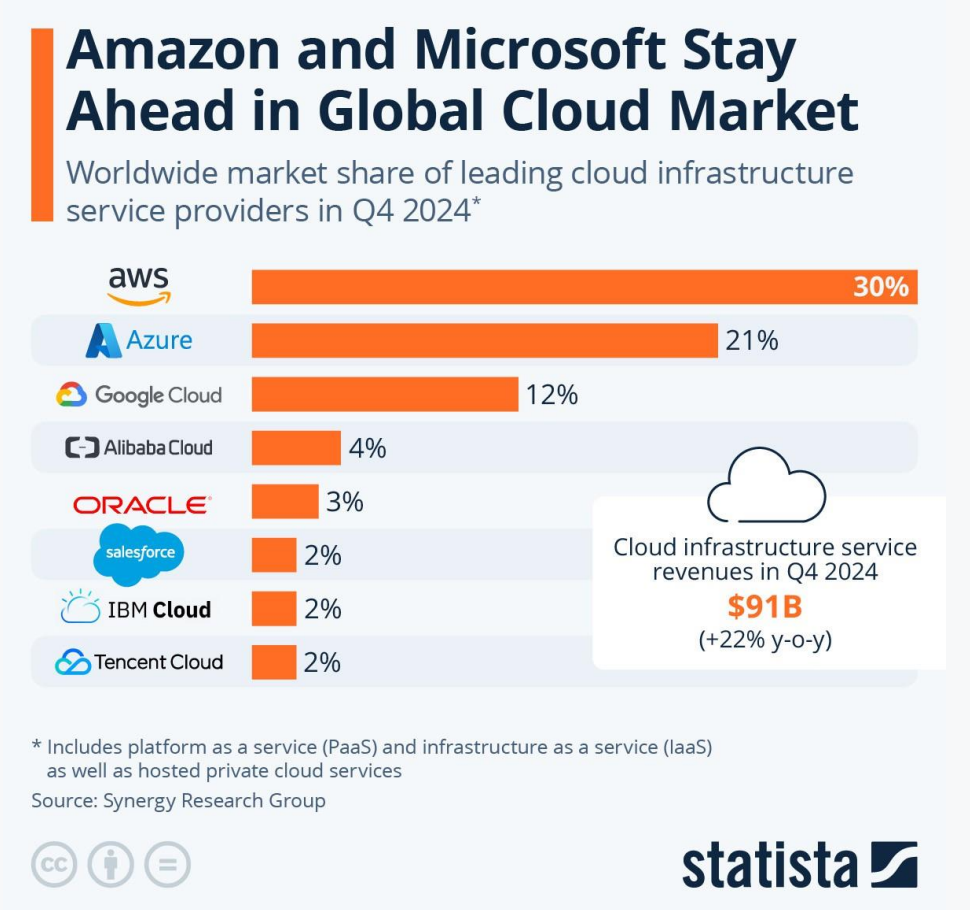
\includegraphics[width=\textwidth]{assets/images/HyperscalerMarketshare}
    \caption{Marktanteil der Cloudprovider.}
\end{figure}         % Anbietervergleich (nutzt Regionen/Zonen)

% Block 4 – Bereitstellung & Services
\section{Cloud Liefermodelle}
\begin{figure}[H]
  \centering
    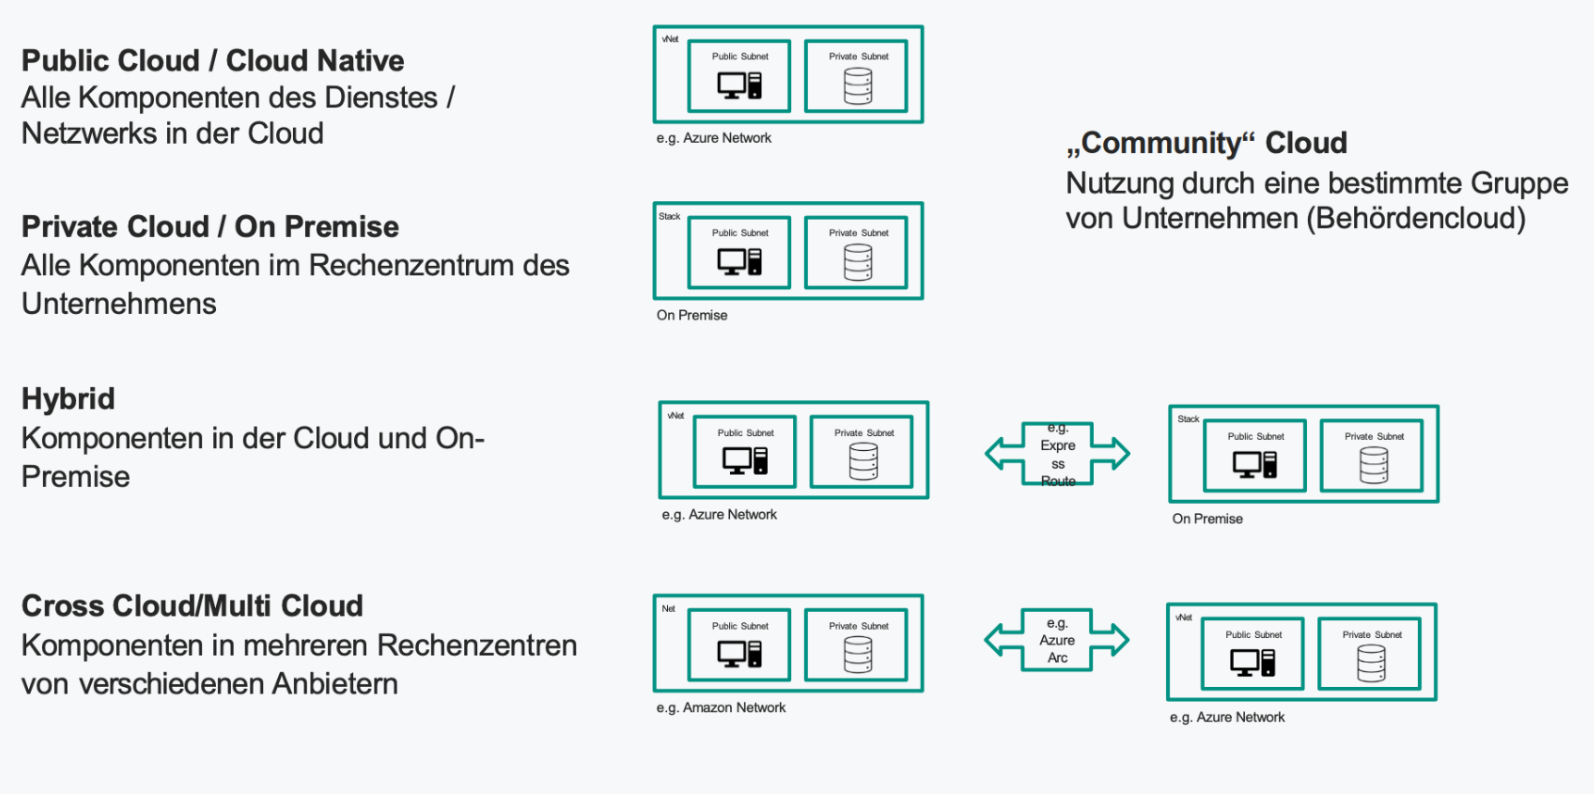
\includegraphics[width=\textwidth]{assets/images/coludliefermodell}
\end{figure}
\begin{table}[H]
    \centering
    \renewcommand{\arraystretch}{1.6}
    \begin{tabular}{|p{2.5cm}|p{2.8cm}|p{3.8cm}|p{3cm}|p{3.2cm}|}
        \hline
        \textbf{Modell}
            & \textbf{Kosten}
            & \textbf{Sicherheit}
            & \textbf{Customization / Flexibilität}
            & \textbf{Notwendige Ressourcen} \\
        \hline
        \textbf{Public Cloud}
            & Kostengünstigste Architektur
            & Hoher Sicherheitsstandard, keine volle Kontrolle (reicht möglicherweise nicht aus)
            & Begrenzt, abhängig vom Dienst des Cloud-Service-Providers (CSP)
            & Kein detailliertes Infrastruktur-Know-how erforderlich \\
        \hline
        \textbf{Private Cloud}
            & Teuerste Architektur
            & Volle Eigenverantwortung: nichts ist vorkonfiguriert, alle Sicherheitsstandards müssen selbst auf eigene Kosten umgesetzt werden
            & Infrastruktur kann beliebig konfiguriert werden
            & Detailliertes Know-how für alle erforderlichen Infrastrukturebenen erforderlich \\
        \hline
        \textbf{Hybride Cloud}
            & Könnte je nach Bedarf Vorteile haben
            & Alle Sicherheitsstandards umsetzbar. Die Verbindung zur Cloud muss gesichert sein
            & Alle Möglichkeiten beider Architekturen
            & Detailliertes Know-how für alle erforderlichen Infrastrukturebenen erforderlich \\
        \hline
    \end{tabular}
    \caption{Vergleich der Cloud-Bereitstellungsmodelle}
    \label{tab:cloud-modelle}
\end{table} % Public/Private/Hybrid
\section{Servicemodelle}

\subsection{Infrastructure as a Service (IaaS)}
Bei \textbf{IaaS} wird dem Nutzer \emph{ausschließlich die Infrastruktur} bereitgestellt.
Ein typisches Beispiel sind virtuelle Maschinen. Der Nutzer ist selbst für
das Betriebssystem und alle darauf installierten Anwendungen verantwortlich.
\textit{Load Balancer} und ähnliche Dienste sind nicht vorkonfiguriert und müssen
manuell eingerichtet werden.

\textbf{Flexibilität:} Hoch, man ist bei der Nutzung vollständig frei.\\
\textbf{Verantwortung:} Hoch, nur die physische Hardware muss nicht selbst
verwaltet werden.\\
\textbf{Typische Anwendungsfälle:} Entwicklungs-Workloads und Hosten von
Legacy-Systemen.
\begin{table}[h]
    \centering
    \begin{tabularx}{\linewidth}{|X|X|X|}
        \hline
        \textbf{Public Cloud} & \textbf{Private Cloud} & \textbf{Hybrid Cloud} \\
        \hline
        IaaS in der Public Cloud wird oft genutzt, um virtuelle Server bereitzustellen, insbesondere für Startups. Zusätzlich ist IaaS in der Public Cloud kostengünstig und skalierbar. & Große Unternehmen können IaaS auch in ihrer Private Cloud nutzen, um maximale Kontrolle über Computing-Ressourcen zu haben. & Die meiste Rechenleistung befindet sich in der Private Cloud, nur bei Spitzenlasten wird auf die Public Cloud gewechselt. Auch Cloud Bursting genannt. \\
        \hline
    \end{tabularx}
\end{table}
\subsection{Platform as a Service (PaaS)}
Bei \textbf{PaaS} bewegt man sich in Richtung \textit{Managed Services}. Ein Beispiel wäre
eine verwaltete SQL-Datenbank in Azure. Viele Aspekte wie Load Balancer und
Skalierung werden bereits vom Anbieter übernommen, was die Entwicklung
deutlich vereinfacht.

\textbf{Flexibilität:} Hoch, allerdings mit deutlich weniger
Konfigurationsaufwand als bei IaaS.\\
\textbf{Verantwortung:} Mittel, viele Dienste werden bereits vom Provider
verwaltet.\\
\textbf{Typische Anwendungsfälle:} Hosten von Webanwendungen, verwaltete
Datenbanken in der Cloud.
\begin{table}[h]
    \centering
    \begin{tabularx}{\linewidth}{|X|X|X|}
        \hline
        \textbf{Public Cloud} & \textbf{Private Cloud} & \textbf{Hybrid Cloud} \\
        \hline
        PaaS wird in der Public Cloud genutzt, um Anwendungen von Entwicklern bereitzustellen. Beispielsweise soll eine Webanwendung für das ganze Unternehmen zur Verfügung gestellt werden – dies wird in Azure beispielsweise über einen Azure App Service getan. & PaaS-Plattformen können auch in einem unternehmenseigenen Rechenzentrum eingerichtet werden, sodass Entwicklungsteams in einer sicheren Umgebung testen können. & Entwicklungsteams testen in einer privaten PaaS-Umgebung und deployen die Anwendung dann in eine öffentliche PaaS-Umgebung. \\
        \hline
    \end{tabularx}
\end{table}
\subsection{Software as a Service (SaaS)}
Bei \textbf{SaaS} erhält der Nutzer ein \emph{fertiges Produkt}, das nur noch konfiguriert
werden muss. Eigener Code kann nicht eingebunden werden, alles funktioniert
über \textit{Customizing}.

\textbf{Flexibilität:} Gering, alles skaliert automatisch, eigene Eingriffe
sind kaum möglich.\\
\textbf{Verantwortung:} Gering, der Nutzer ist nur für die eigenen Daten
verantwortlich.\\
\textbf{Typische Anwendungsfälle:} Produkte wie Microsoft 365.
\begin{table}[h]
    \centering
    \begin{tabularx}{\linewidth}{|X|X|X|}
        \hline
        \textbf{Public Cloud} & \textbf{Private Cloud} & \textbf{Hybrid Cloud} \\
        \hline
        SaaS-Produkte wie Microsoft 365, Gmail oder Salesforce sind am weitesten verbreitet. Eine Anwendung läuft komplett in der Public-Cloud-Infrastruktur eines Anbieters. Die Anwendungen werden über das Internet bereitgestellt. & SaaS-Produkte können bei Unternehmen mit hohen Sicherheitsanforderungen in der eigenen Cloud-Infrastruktur gehostet werden. Beispielsweise können auch KI-Modelle wie Claude oder Gemini bei einem Unternehmen selbst gehostet werden. & Dies ist eine häufige Kombination in Unternehmen: Sensible Daten liegen On-Premises in der Private Cloud, beispielsweise auch ein ERP-System. Daneben werden aber auch SaaS-Anwendungen wie Teams oder Gmail genutzt. \\
        \hline
    \end{tabularx}
\end{table}
\newpage
\subsection{Shared Responsibility Model}
Das \textbf{Shared Responsibility Model} zeigt auf, wo die Verantwortlichkeiten bei
Cloud-Modellen liegen und wie viel vom Nutzer bzw. Unternehmen selbst
gemanagt werden muss im Vergleich zu dem, was der Cloud-Provider übernimmt.

\begin{figure}[H]
    \centering
    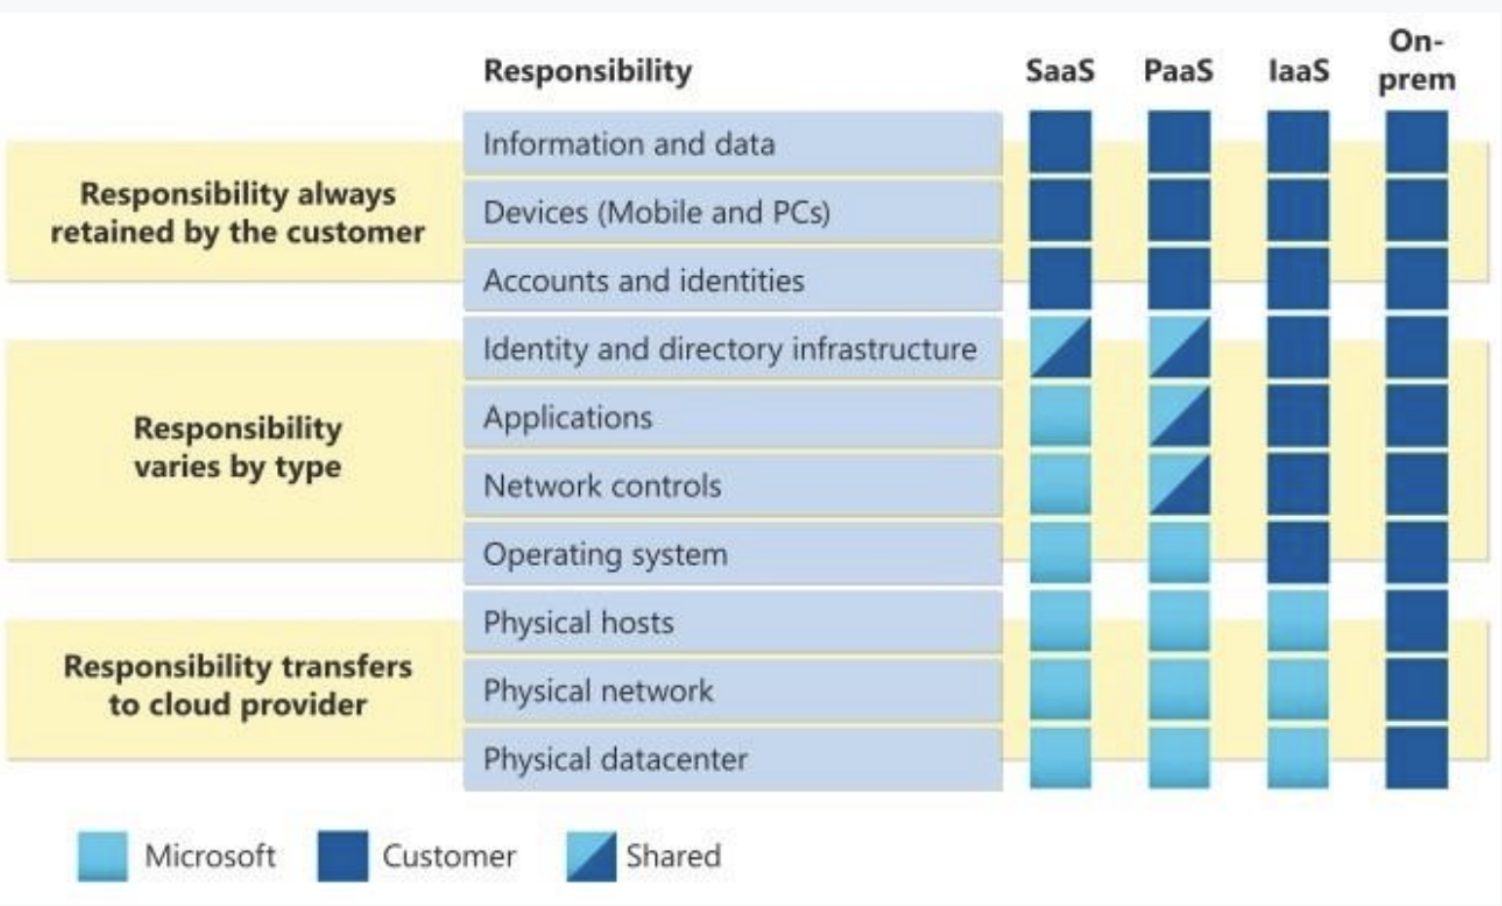
\includegraphics[width=\textwidth]{assets/images/SharedResponbility}
    \caption{Shared Responsibility Model}
\end{figure}

\subsubsection{Sicherheitsaufgaben von Kunde und Provider}
Der Kunde ist hauptsächlich für die Sicherheit der Client-Geräte
verantwortlich, also beispielsweise dafür, dass Mitarbeiter sichere
Passwörter verwenden. Zusätzlich können \textit{RBAC} und \textit{Conditional Access}
aktiviert werden, sodass Endnutzer automatisch mehr Sicherheit erhalten.
Authentifizierung, die beispielsweise \textit{SSO} ermöglicht, wird vom Cloud-Provider
bereitgestellt. Der Provider ist seinerseits vollständig für die Sicherheit
im Rechenzentrum und seiner eigenen Services zuständig. Für die Sicherheit
der eigenen Daten ist der Kunde verantwortlich, muss dafür aber oft nur
wenige Konfigurationen vornehmen, beispielsweise Disaster Recovery durch
Zonenredundanz.

\subsubsection{Warum verändern sich die Verantwortlichkeiten?}
Die verschiedenen Servicemodelle haben unterschiedliche Anwendungsfälle.
IaaS wird genutzt, wenn möglichst viel selbst konfiguriert werden soll,
beispielsweise für das Hosten von Legacy-Systemen oder Entwicklungs-Workloads.
Die Kosten für den Compute werden dabei oft im Voraus bezahlt, beispielsweise
über \textit{Azure Reservations}. PaaS wird für eigene Cloud-Native-Anwendungen
genutzt, hat aber grundlegende Dinge bereits vorkonfiguriert, sodass keine
VM manuell eingerichtet werden muss. SaaS sind vollständig abgeschlossene
Softwareprodukte, die einfach über die Cloud laufen, wie beispielsweise
Microsoft 365.     % IaaS/PaaS/SaaS + Shared Responsibility
\section{Cloud Services}
Ein Cloud-Dienst (englisch: Cloud Service) bezeichnet eine Dienstleistung, die von einem Cloud-Provider über das Internet bereitgestellt wird. Dabei stellt der Anbieter Ressourcen wie Compute, Speicher oder Software auf Abruf zur Verfügung, ohne dass der Nutzer eigene physische Infrastruktur betreiben muss.
\begin{figure}[H]
    \centering
    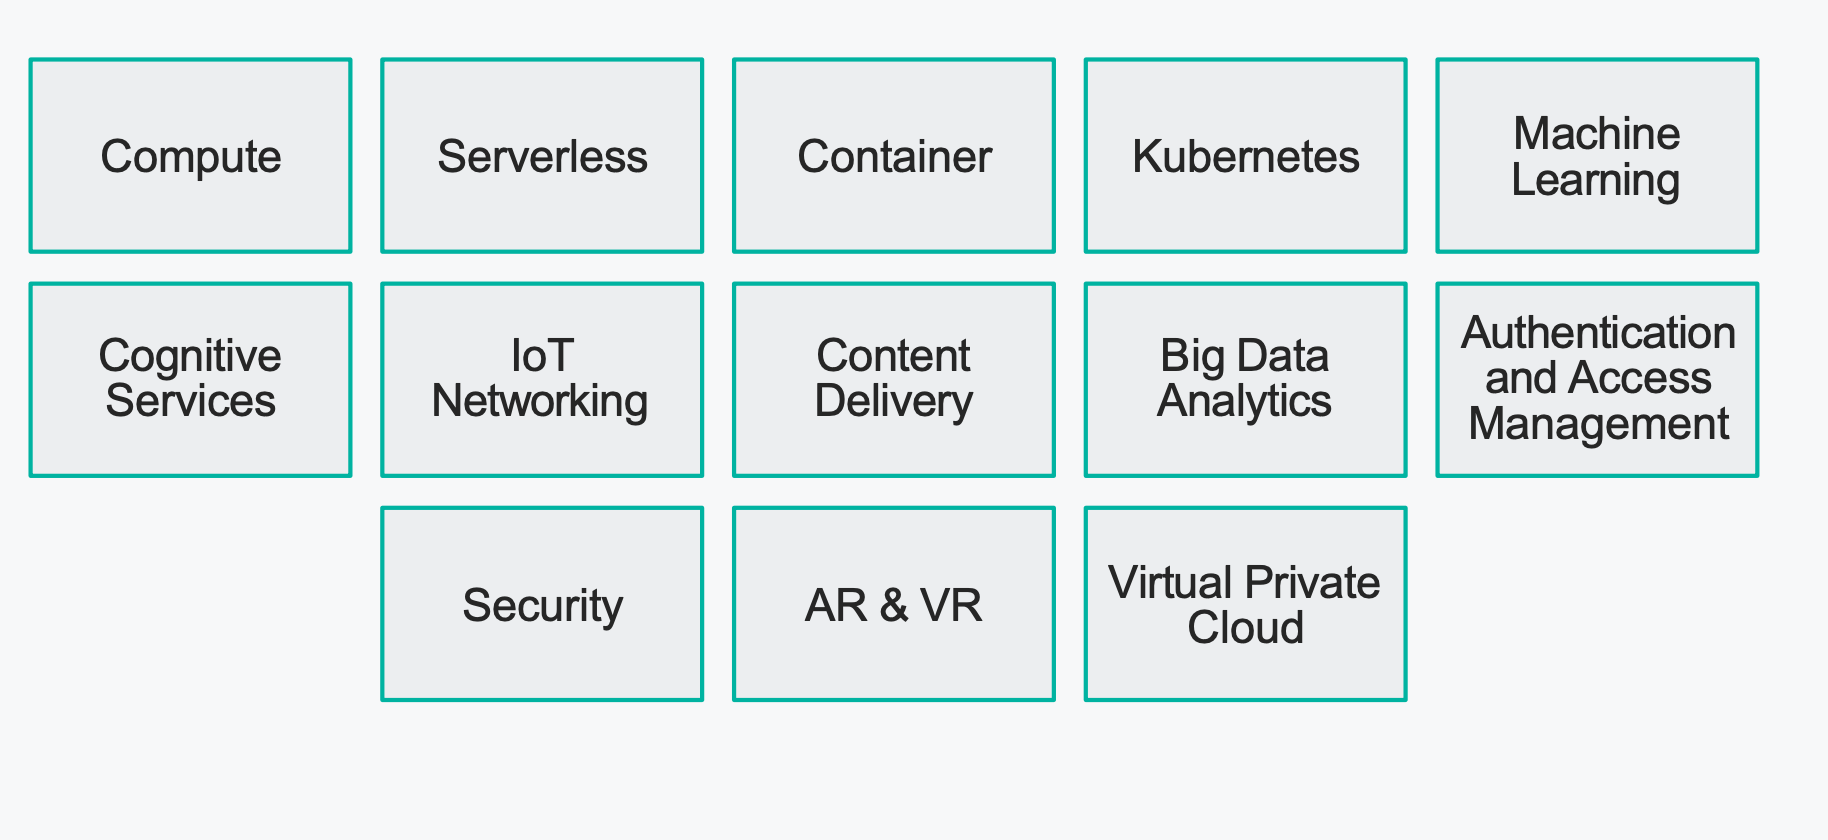
\includegraphics[width=\textwidth]{assets/images/TypischeCloudService}
    \caption{Grundlegende Services in Der Cloud}
\end{figure}
\subsection{Compute}
Compute bedeutet das bereitstellen von Rechenleistung. Also kann Compute hosten einer Webanwendung bedeutet oder des hosten eine KI modell wie Sonnet oder GPT 5 für ein Unternehmen.
\subsection{Serveless}
Serveless bedeutet das man Code ohne Pflege eines Server Hosten kann. Es ist oft teil von Ressourcen in Azure z.B. der Managed Service für Postgre Datenbanken. Ein sonder fall ist FaaS. Dies wird Später noch mal detailert erklärt.
  \begin{infobox}[Definiton FaaS – Function as a Service]
    FaaS baut auf Serveless auf und emrölicht Backend cod Serveless zu hosten, Durch Genreische sprachen wie z.B. Python. 
  \end{infobox}
\begin{table}[H]
  % \caption kommt VOR der Tabelle (FOM-Konvention)
  
  \label{tab:server-vs-serverless}

  % tabularx: streckt die Tabelle auf \textwidth
  % l = linksbündig, feste Breite (Aspekt-Spalte)
  % X = flexibel, füllt den Rest (die zwei Inhalts-Spalten)
  \begin{tabularx}{\textwidth}{|l|X|X|}
    \hline
    \textbf{Aspekt}
      & \textbf{Server Architecture}
      & \textbf{Serverless Architecture} \\
    \hline

    Infrastructure Management
      & Entwickler verwalten zugrunde liegende Server oder VMs.
      & Der Cloud-Anbieter verwaltet die Infrastruktur (Server). \\
    \hline

    Resource Allocation
      & Ressourcen, die basierend auf dem erwarteten Workload bereitgestellt werden.
      & Ressourcen, die dynamisch basierend auf dem Bedarf zugewiesen werden. \\
    \hline

    Scaling
      & Die Skalierung umfasst in der Regel manuelle oder automatisierte Prozesse.
      & Automatische Skalierung basierend auf Workload. \\
    \hline

    Cost Model
      & Die Kosten beinhalten Vorabinvestitionen und das laufende Management.
      & Pay-per-Use-Preismodell basierend auf Funktionsaufrufen. \\
    \hline

    State Management
      & Anwendungen behalten den Status auf der Serverseite bei.
      & Serverlose Funktionen sind von Natur aus zustandslos. \\
    \hline

  \end{tabularx}
  \caption{Vergleich Server Architecture und Serverless Architecture}

\end{table}
     % Überblick/Brücke: Compute, Storage, Serverless
\subsection{Serverless}
Serverless ist in der Cloud die Möglichkeit, ohne einen eigenen Server Services und Code zu hosten. Bei Serverless muss man selbst keine Server mehr verwalten oder Code builden und laufen lassen. Man deployed den Code einfach und die Cloud führt den Code aus – natürlich nur, wenn dieser fehlerfrei ist. Durch eine CI/CD-Pipeline kann man beispielsweise bei einem Git-Commit auf einen Branch das Builden eines Docker-Images automatisieren; dieses wird dann automatisch in einer Registry hinterlegt.

\subsection{Function as a Service – FaaS}
Function as a Service ist Teil des PaaS-Modells und ist besonders eng mit Serverless verwoben. Bei Function as a Service wird Code mit Business-Logik – also Backend-Code – in der Cloud deployed.
Meist sind dies einzelne Funktionen. Diese Funktionen werden beim FaaS-Modell automatisch horizontal skaliert. Sie werden durch Events getriggert, beispielsweise durch HTTP-Requests, AWS S3 oder auch Webhooks. Das Deployment bei FaaS ist sehr einfach, da man wirklich nur Code ablegen muss.
FaaS-Services heißen bei Azure Azure Functions, bei AWS AWS Lambda und bei Google Google Cloud Functions. Open-Source-Alternativen sind OpenFaaS, Nuclio, Fn, Kubeless, Fission und Apache OpenWhisk.
\begin{figure}[H]
  \centering
  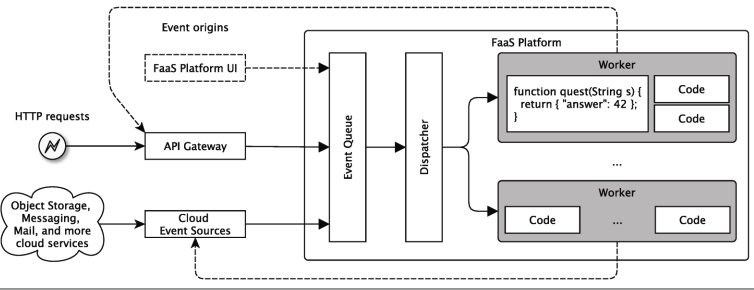
\includegraphics[width=\textwidth]{assets/images/FaaS_Architektur}
  \caption{Architektur von FaaS}
\end{figure}
\begin{table}[H]
  \caption{Vergleich Server- und Serverless-Architektur}\label{tab:server-serverless}
  \begin{tabularx}{\textwidth}{|l|X|X|}  % Spalte 1 fest linksbuendig, Spalte 2+3 fuellen Rest gleichmaessig
    \hline
    \textbf{Aspekt} & \textbf{Server Architecture} & \textbf{Serverless Architecture} \\
    \hline
    \textbf{Infrastructure Management} & Entwickler verwalten zugrunde liegende Server oder VMs. & Der Cloud-Anbieter verwaltet die Infrastruktur (Server). \\
    \hline
    \textbf{Resource Allocation} & Ressourcen, die basierend auf dem erwarteten Workload bereitgestellt werden. & Ressourcen, die dynamisch basierend auf dem Bedarf zugewiesen werden. \\
    \hline
    \textbf{Scaling} & Die Skalierung umfasst in der Regel manuelle oder automatisierte Prozesse. & Automatische Skalierung basierend auf Workload. \\
    \hline
    \textbf{Cost Model} & Die Kosten beinhalten Vorabinvestitionen und das laufende Management. & Pay-per-Use-Preismodell basierend auf Funktionsaufrufen. \\
    \hline
    \textbf{State Management} & Anwendungen behalten den Status auf der Serverseite bei. & Serverlose Funktionen sind von Natur aus zustandslos. \\
    \hline
  \end{tabularx}
\end{table}
\subsubsection{Entwicklung von FaaS}
Die Entwicklung für FaaS läuft in 6 Phasen ab:
\begin{itemize}
  \item Design: Das ist die Entwurfsphase, in der festgelegt wird, was die Funktion tun soll. Gerade bei FaaS gibt es einiges zu beachten, wie beispielsweise das Double-Spending-Problem.
  \item Code: Man implementiert das Design in Code.
  \item Lokal getestet: Testen des Codes in der lokalen Umgebung. Meist wird hier nur getestet, ob das Programm das ausgibt, was es soll, ob es kompiliert und welche Laufzeit es hat. Andere Tests sind gerade bei Serverless schwer durchzuführen.
  \item Integrationstests: Tests in einer Cloud-Umgebung, meist auch in einer Produktionsumgebung.
  \item Deploy: Den Code in die Cloud bringen.
  \item Monitor: Man betrachtet, wie der Output der Funktion ist und wie diese in der Cloud funktioniert und performt. Gegebenenfalls gibt es Änderungen an der Funktion.
\end{itemize}
\subsubsection{Limitationen von Serverless}
\begin{figure}[H]
  \centering
  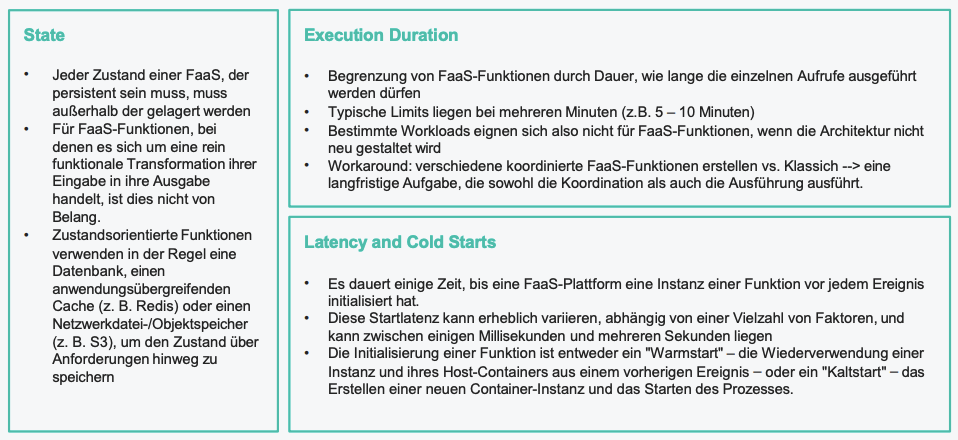
\includegraphics[width=\textwidth]{assets/images/ServelessLimit}
  \caption{Limitation von Serverless}
\end{figure}
\subsubsection{FaaS und Abrechnungen: Das Double-Spending-Problem}
Bei FaaS wird mit Pay-as-you-go-Preisen gerechnet bzw. Pay-by-the-Millisecond, also sollte die Laufzeit des Programms optimiert sein.
Ein Problem, das gerade wegen Pay-by-the-Millisecond auftauchen kann, ist das \textbf{Double-Spending-Problem}. Das tritt auf, wenn eine Funktion eine andere Funktion aufruft, denn dann arbeiten beide gleichzeitig und man muss für beide gleichzeitig bezahlen, da man für zwei Laufzeiten gleichzeitig zahlt. Dies sollte man beim Erstellen von Functions immer in Betracht ziehen.
\begin{figure}[H]
  \centering
  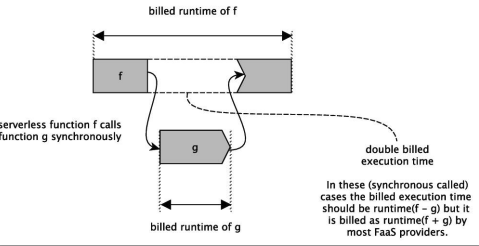
\includegraphics[width=\textwidth]{assets/images/DoubleSpendingProblem}
  \caption{Double Spending}
\end{figure}
         % Serverless & FaaS im Detail

% Block 5 – Anwendungen bauen
\section{Docker und Kubernetes}

\subsection{Docker}
\textbf{Docker} ist eine \emph{Containerisierungs-Plattform}. Sie erlaubt es, Anwendungen zusammen mit allem, was sie zum Laufen brauchen, in sogenannte Container zu verpacken. Vor Containern gab es oft den Spruch "Works on my Machine", da ein Entwickler andere Abhängigkeiten installiert hatte als der andere Kollege. Das Problem ist durch Docker gelöst, da man alle Abhängigkeiten mitgibt.

\subsubsection{Image}
Ein \textbf{Image} ist der \textit{Blueprint}, also die Vorlage für einen Container. Es enthält alles, was zum Ausführen eines Containers erforderlich ist. Ein Image kann in einer \textit{Docker Compose} referenziert werden. In dieser werden auch noch Einstellungen vorgenommen wie Environment-Variablen.

Beispiel einer Docker Compose, mit der MySQL ausgeführt wird:

\begin{syntaxbox}[YAML]
services:
  mysql:
    image: mysql:8.0
    container_name: mysql_dev
    restart: unless-stopped

    command:
      - --default-authentication-plugin=mysql_native_password
      - --bind-address=0.0.0.0

    ports:
      - "3307:3306"

    environment:
      MYSQL_ROOT_PASSWORD: Levin-Dev-SQL

    volumes:
      - mysql_data:/var/lib/mysql
      - ./init.sql:/docker-entrypoint-initdb.d/init.sql

volumes:
  mysql_data:
\end{syntaxbox}

\subsubsection{Container}
Ausführbare Pakete mit Anwendungscode, Laufzeit, Bibliotheken und Abhängigkeiten. Sie sind \emph{zustandslos und unveränderlich}. Bei Code-Änderungen müssen sie neu erstellt werden.

\subsubsection{Container Registry}
Eine \textbf{Container Registry} ist der Ort, an dem Images gespeichert werden. Es gibt öffentliche Registries wie beispielsweise \textit{Docker Hub}, aber auch jeder Cloud-Anbieter bietet die Möglichkeit, eine eigene unternehmensinterne Container Registry zu hosten.

\subsection{Kubernetes}
\textbf{Kubernetes} oder auch \textit{K8s} wurde von Google entwickelt. Kubernetes ist eine Plattform, um Container zu \emph{orchestrieren}. Es verwaltet Container (nicht nur von Docker). Durch Kubernetes sind \emph{Hochverfügbarkeit}, \emph{Skalierbarkeit} und \emph{Disaster Recovery} möglich.

\begin{figure}[H]
    \centering
    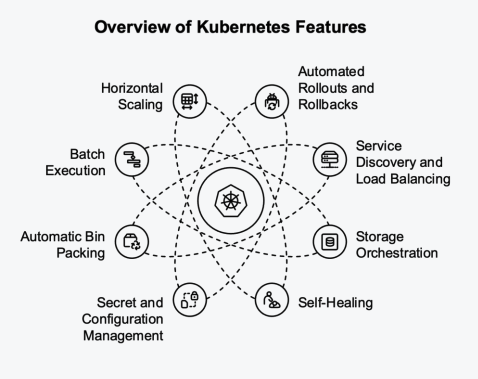
\includegraphics[width=\textwidth]{KubernetsFeatures}
    \caption{Kubernetes Features}
\end{figure}

\subsubsection{Pods}
Ein \textbf{Pod} ist die \emph{kleinste Einheit} in Kubernetes. Ein Pod kann aus einem oder mehreren Containern bestehen. Alle Container in einem Pod haben geteilte Ressourcen wie Speicher und Netzwerk. Beispielsweise kann eine App in einem App-Pod zusammengefasst werden.

\subsubsection{Node}
Ein \textbf{Node} ist ein Server bzw. Rechner eines Clusters.

\subsubsection{Cluster}
Ein \textbf{Cluster} ist eine Sammlung von Nodes, die gemeinsam Container und Pods ausführen.

\subsubsection{Instanzen}
Eine einzelne laufende Kopie einer Ressource.

\subsubsection{Deployments}
Vergleichbar mit \textit{Docker Compose}. Ein \textbf{Deployment} enthält mehrere Container und ist sozusagen ein Bauplan für einen Pod. Allerdings wird auch angegeben, wie viele Pods existieren sollen.

\subsubsection{Services}
Ein \textbf{Service} ist die \emph{stabile Netzwerk-Abstraktion} vor einer Menge von Pods, die den Traffic an diese Pods weiterleitet. Er stellt eine stabile IP und einen Port bereit und kann Funktionen wie einen \textit{Load Balancer} konfiguriert haben, sodass die dahinterliegenden Pods erreichbar bleiben, auch wenn sie sich ändern.

\subsection{Kubernetes Funktion}
Ein Kubernetes Cluster benötigt eine \textit{Master Node}. Diese wird zur \textit{Control Plane}, die die Container auf den \textit{Worker Nodes} verwaltet. Wenn ein Node ausfällt, hat Kubernetes die \textit{Self-Healing}-Funktion und führt den Container auf einem anderen Node aus. Ein Cluster hat ein virtuelles Netzwerk, damit die Nodes untereinander kommunizieren können.
\section{Cloud Native}
Der Begriff \textbf{Cloud Native} wurde 2013 von Matt Stine geprägt und unter anderem durch Netflix auf einem AWS re:Invent Talk bekannt gemacht. Es gibt keine einheitliche Definition für Cloud-Native-Architektur. Grundsätzlich soll Cloud Native dabei helfen, Webanwendungen zu entwickeln, die \emph{skalierbar} und \emph{hochverfügbar} sind. Gleichzeitig soll durch Cloud Native \emph{agil} entwickelt werden, also eine schnellstmögliche Feature-Anpassung mit möglichst kleinem Risiko. Dabei helfen \textit{Microservices} statt einer monolithischen Architektur, \textit{Container}, \textit{DevOps} sowie \textit{CI/CD-Pipelines}. Viele Lösungen wie Komponenten, \textit{Logging} und \textit{Tracing} sind dabei standardisiert.
\begin{figure}[H]
    \centering
    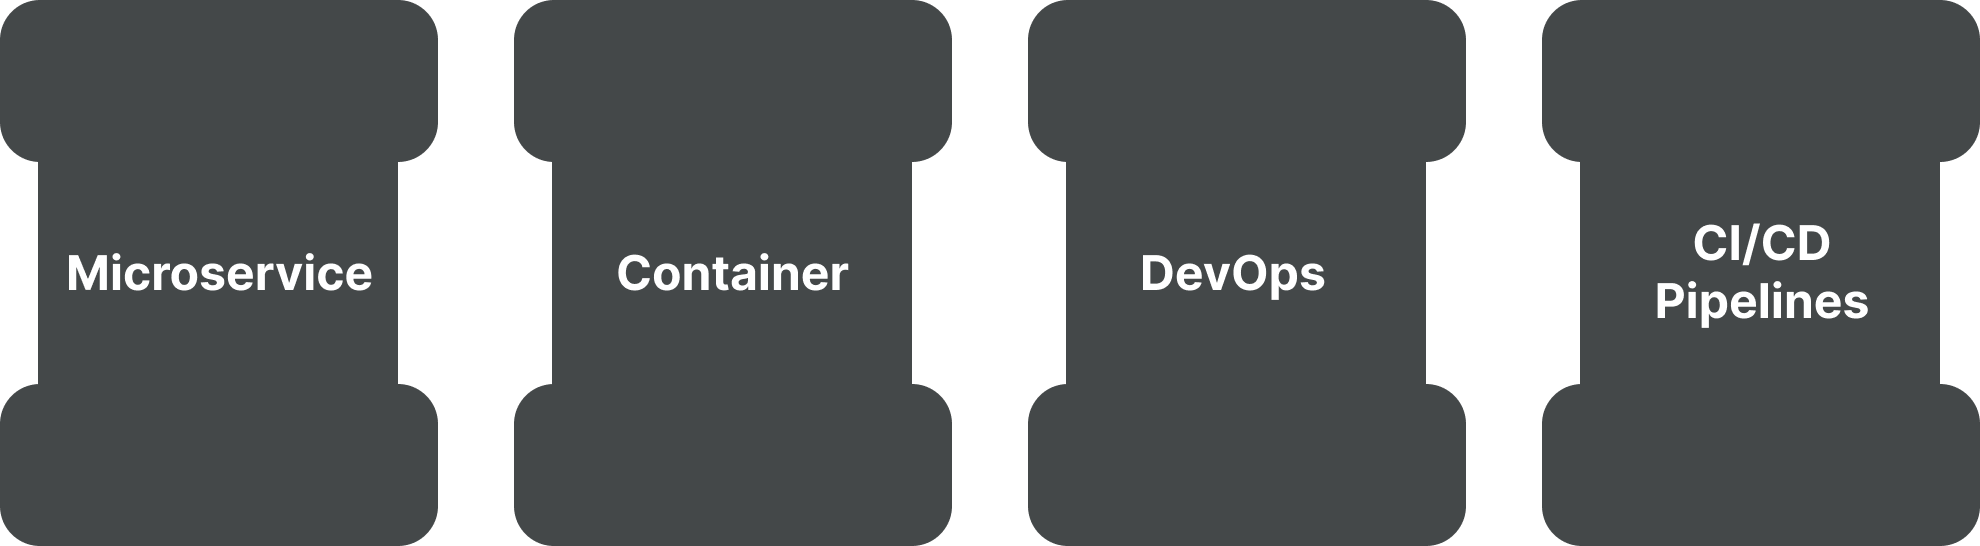
\includegraphics[width=\textwidth]{CloudNativeSaulen.png}
    \caption{Die 4 Saulen von Cloud Native}
\end{figure}

\begin{figure}[H]
    \centering
    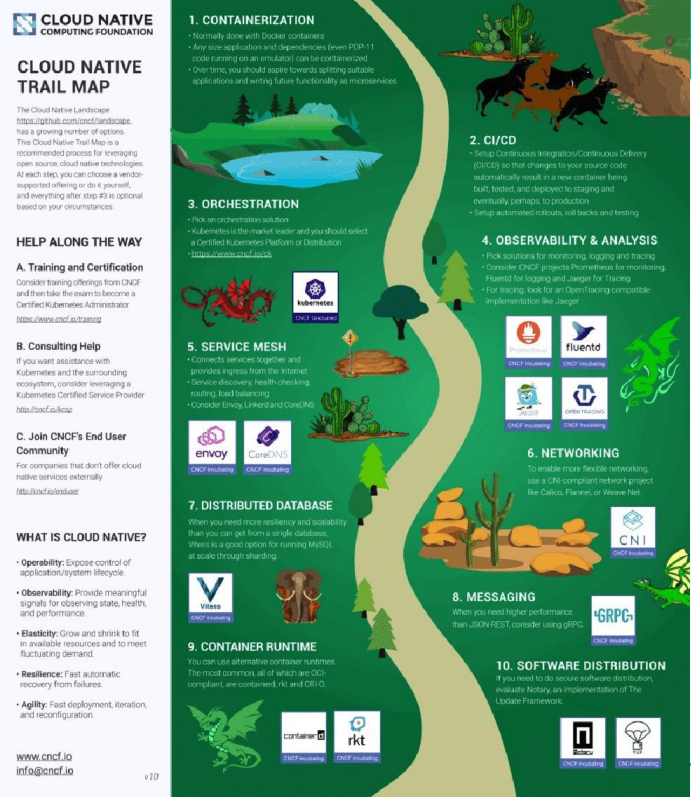
\includegraphics[width=\textwidth]{CloudNativeMap.png}
    \caption{Cloud Native Landscape (CNCF)}
\end{figure}

\subsection{DevOps}
Kombination aus \textit{Development} und \textit{Operations}.
Entwicklung und Betrieb arbeiten \emph{zusammen statt getrennt}.
\textbf{Kern-Ideen:} Automatisierung von Builds, Tests und Deployments,
schnelle Feedbackschleifen (kurze Release-Zyklen) und gemeinsame
Verantwortung für Code und Infrastruktur.

\subsection{CI/CD -- Continuous Integration / Continuous Delivery}
\textbf{CI:} Jeder Code-Push wird automatisch gebaut und getestet,
Fehler werden sofort sichtbar.
\textbf{CD:} Nach erfolgreichem CI wird der Build automatisch
in eine Umgebung ausgeliefert (Staging oder Produktion).

\subsection{Microservices}
Architekturstil, bei dem eine Anwendung in viele kleine, unabhängige
Dienste aufgeteilt wird. Jeder Service hat eine \emph{klar abgegrenzte Aufgabe},
kommuniziert über \textit{APIs} (REST oder Message Queues) und kann separat
deployt und skaliert werden. Gegenteil: \textit{Monolith}.

\subsection{Monolith}
Eine monolithische Architektur bedeutet, dass alle Elemente einer Software in einer
zusammenhängenden Codebasis liegen. Die grafische Benutzeroberfläche, die Geschäftslogik
und der Datenzugriff sind eng miteinander verbunden. Dies führt dazu, dass die Codebasis
stark anwächst, wodurch Fehler schwerer nachvollziehbar werden. Bereits eine kleine
Änderung erfordert, dass die gesamte Anwendung neu deployt wird. Die beteiligten Teams
sind häufig groß und müssen bereichsübergreifend zusammenarbeiten.

\begin{figure}[H]
    \centering
    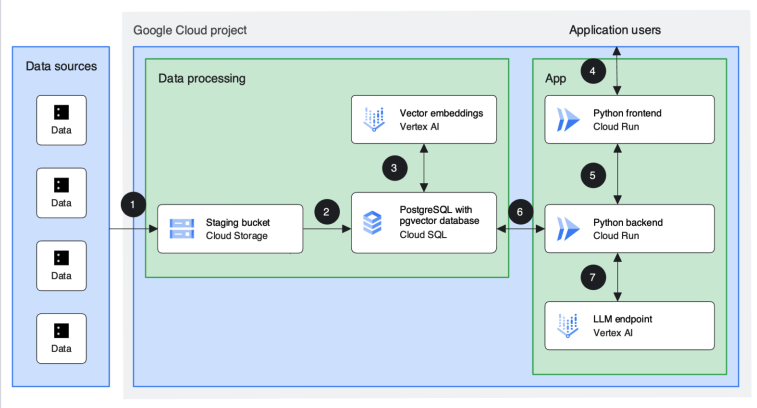
\includegraphics[width=\textwidth]{CloudNativeBesipel.png}
    \caption{Microservices vs.\ Monolith}
\end{figure}
            % Cloud Native, DevOps, CI/CD, Microservices
\section{Architektur-Grundlagen \& Frameworks}

\subsection{Warum wichtig?}
Pläne beeinflussen spätere Entscheidungen. Viele Änderungsanfragen
sind vermeidbar, sonst entstehen \emph{technische Schulden}. Framework-Änderungen
allein lösen keine Grundprobleme, und eingeschränkte Komponentenwahl
wirkt sich auf Folgeprojekte aus (z.\,B. Lizenzen).

\subsection{Technische Schulden}
\textbf{Definition:} Konsequenzen bei schlechter Umsetzung.\\[4pt]
\textbf{Arten:}
\begin{itemize}
    \item Bewusste Schulden (strategische Entscheidungen)
    \item Unbeabsichtigte Schulden durch mangelnde Dokumentation,
          fehlende Automatisierung, fehlende Coding Standards
          oder Missachtung von Code-Hinweisen
\end{itemize}

\subsection{Ziele einer Lösungs-Architektur}
\begin{itemize}
    \item Skalierbarkeit, Resilienz, Sicherheit, Compliance
    \item Globaler Kundendienst mit gleicher Performance
    \item Wartbarkeit über Jahrzehnte
\end{itemize}

\subsection{Architektur-Perspektiven}
\begin{itemize}
    \item \textbf{Geschäftssicht:} Ziele, Vision, Stakeholder,
          Geschäftsanforderungen, Erfolgsmetriken
    \item \textbf{Prozesssicht:} Abläufe von Kunde zu Server,
          z.\,B. als Sequenzdiagramm oder BPMN
    \item \textbf{Konzeptionelle Sicht:} Architektur ohne
          spezifische Cloud-Provider-Komponenten
    \item \textbf{Lösungssicht:} Cloud-Service-Architektur,
          User Flow, ER-Diagramm
    \item \textbf{Sicherheitssicht:} Zugangsverwaltung,
          Compliance-Anforderungen, Firewall
\end{itemize}

\newpage

\subsection{Architektur-Frameworks: Governance}
Dienen der unternehmensweiten Steuerung, Compliance-Nachweisen
und Risikokontrolle über vordefinierte Prinzipien, Gremien und Reviews.
Beispiele: \textit{TOGAF}, \textit{ISO/IEC/IEEE 42010:2022}, \textit{Zachman-Framework}.\\[4pt]
\textbf{TOGAF} (The Open Group Architecture Framework): Framework zur
Entwicklung und Verwaltung von Unternehmensarchitekturen (People,
Processes, Technology) mit vier Architektur-Domänen:
% LEKTORAT (fachlich): Vorher als "vier Domänen" angekündigt, aber nur drei
% gelistet. TOGAF unterscheidet vier Domänen; die Informationssystem-
% architektur zerfällt in Anwendungs- und Datenarchitektur.
\begin{itemize}
    \item Geschäftsarchitektur (Business)
    \item Datenarchitektur (Data)
    \item Anwendungsarchitektur (Application)
    \item Technologiearchitektur (Technology)
\end{itemize}

\subsection{Architektur-Frameworks: Praxisorientiert}
Stellen schnelle, verständliche Diagramme für Entwickler, DevOps und
Produktteams bereit. Zielen eher auf einzelne Lösungen und Applikationen
ab. Beispiele: \textit{C4-Modell}, \textit{4+1-Modell}, \textit{PlantUML}.\\[4pt]
\textbf{C4-Modell:} Unterstützt Software-Entwicklungsteams, ihre
Architektur bei Planung und Durchführung zu erklären.
4 Ebenen: Software System, Container, Component, Code.\\[4pt]
\textbf{Software Architecture Diagramming Maturity Model:}
\begin{itemize}
    \item \textbf{Level 1 -- Initial:} Keine Architekturdiagramme
    \item \textbf{Level 2 -- Ad hoc:} Diagramme mit ad-hoc-Abstraktionen
          in einem allgemeinen Diagramm-Tool
    \item \textbf{Level 3 -- Defined:} Diagramme mit definierten
          Abstraktionen und Notation, allgemeines Tool
    \item \textbf{Level 4 -- Modelled:} Definierte Abstraktionen in
          einem Modellierungs-Tool, manuell erstellt
    \item \textbf{Level 5 -- Optimising:} Modellelemente werden
          teamübergreifend geteilt, als querybare Datensätze genutzt
          und automatisch aus Sourcecode bzw. Deployment-Umgebung
          generiert
\end{itemize}

\subsection{Frameworks im Detail (TOGAF \& C4)}
\subsubsection{TOGAF -- Architecture Development Method (ADM)}
\begin{figure}[H]
    \centering
    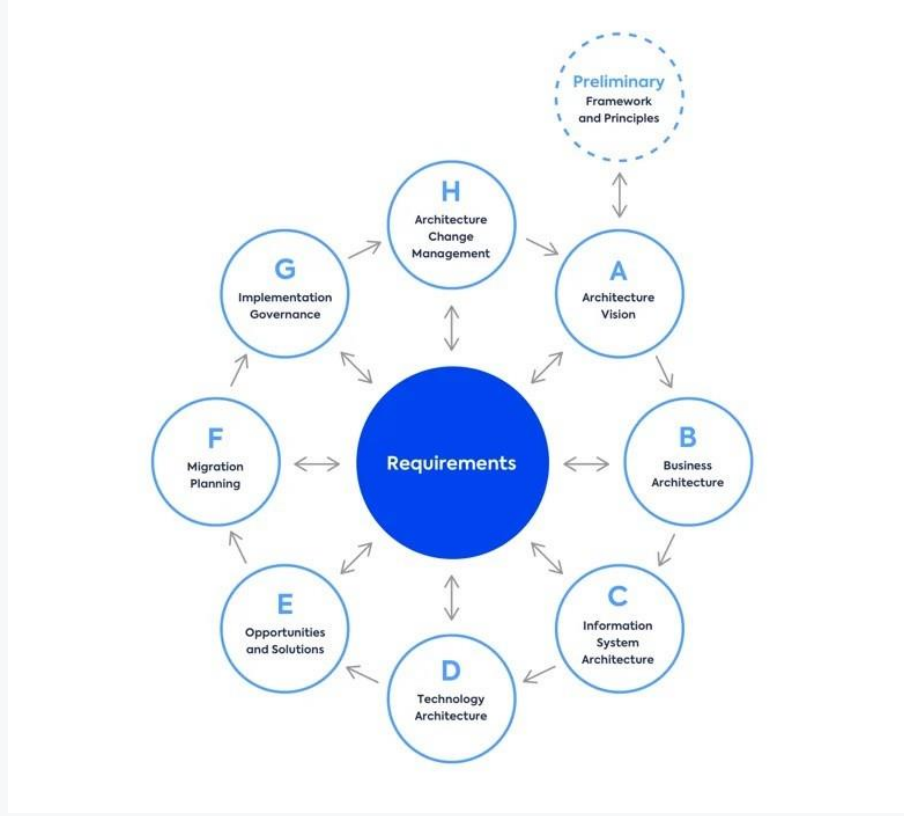
\includegraphics[width=\textwidth]{TOGAF.png}
    \caption{TOGAF ADM-Zyklus}
\end{figure}

Der ADM-Zyklus beschreibt, wie eine Unternehmensarchitektur schrittweise
entwickelt wird. Im Zentrum stehen immer die \textbf{Requirements} (Anforderungen),
auf die jede Phase kontinuierlich einzahlt.

\begin{itemize}
    \item \textbf{Preliminary:} Framework und Prinzipien festlegen
          (Vorbereitung, noch kein offizieller Buchstabe)
    \item \textbf{A -- Architecture Vision:} Ziele, Scope und
          Stakeholder-Erwartungen definieren
    \item \textbf{B -- Business Architecture:} Geschäftsprozesse
          und -strukturen modellieren
    \item \textbf{C -- Information System Architecture:}
          Anwendungs- und Datenarchitektur beschreiben
    \item \textbf{D -- Technology Architecture:} Infrastruktur,
          Plattformen und Technologien festlegen
    \item \textbf{E -- Opportunities \& Solutions:} Lücken zwischen
          Ist- und Soll-Zustand identifizieren, Lösungsoptionen bewerten
    \item \textbf{F -- Migration Planning:} Roadmap und Reihenfolge
          der Umsetzung planen
    \item \textbf{G -- Implementation Governance:} Umsetzung
          begleiten und sicherstellen, dass Architekturvorgaben
          eingehalten werden
    \item \textbf{H -- Architecture Change Management:} Änderungen
          am laufenden System kontrolliert einführen und den
          Zyklus bei Bedarf neu starten
\end{itemize}

Der Zyklus ist \textbf{iterativ}, d.\,h. nach Phase H kann der Prozess
wieder bei A (oder sogar Preliminary) beginnen, falls sich Anforderungen
grundlegend ändern.

\subsubsection{C4}

Das C4-Modell ist ein praxisorientiertes Framework zur Visualisierung
von Software-Architektur. Der Name steht für die vier Abstraktionsebenen:
\textbf{Context, Container, Component und Code}. Die Idee dahinter ist,
dass verschiedene Zielgruppen unterschiedliche Detailtiefe brauchen,
ein Manager braucht nur den groben Überblick, ein Entwickler hingegen
die genaue Komponentenstruktur.
\begin{figure}[H]
    \centering
    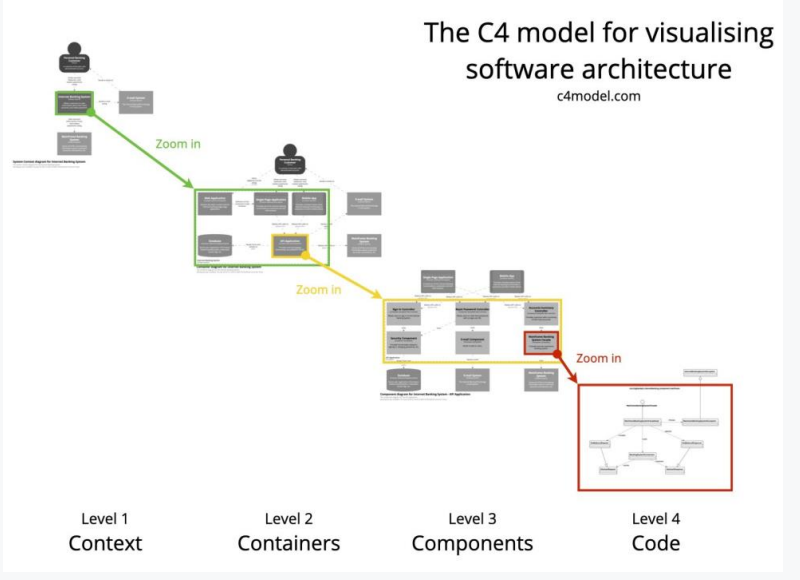
\includegraphics[width=\textwidth]{c4.png}
    \caption{C4-Modell -- vier Abstraktionsebenen}
\end{figure}

Die vier Ebenen bauen aufeinander auf:
\begin{itemize}
    \item \textbf{System Context:} Zeigt das System als Ganzes
          und seine Beziehungen zu Nutzern und externen Systemen
    \item \textbf{Container:} Aufschlüsselung in deploybare Einheiten
          wie Web-Apps, Datenbanken oder Microservices
    \item \textbf{Component:} Interne Struktur eines Containers,
          z.\,B. einzelne Module oder Services
    \item \textbf{Code:} Klassendiagramme oder ähnliches auf
          Code-Ebene (wird selten gezeichnet, da IDEs das übernehmen)
\end{itemize}

Ein großer Vorteil des C4-Modells ist die \textbf{Werkzeugfreiheit}.
Es funktioniert mit PlantUML, draw.io oder sogar auf einem Whiteboard,
solange die vier Ebenen klar getrennt bleiben.
 % Grundlagen + Frameworks (TOGAF, C4)
\section{Architektur-Patterns}

\subsection{Load Balancer}
Die Hauptaufgabe eines \textbf{Load Balancers} ist der \emph{Lastenausgleich}. Wenn viele Nutzer Anfragen an eine Anwendung stellen, werden diese auf mehrere Server verteilt. Dadurch werden Über- und Unterlastung von Ressourcen vermieden. Die meisten PaaS-Angebote in der Cloud kommen mit einem vorkonfigurierten Load Balancer. Bei einem Load Balancer skaliert man \emph{horizontal} (mehr Instanzen, nicht stärkere Hardware).

Weitere Funktionen eines Load Balancers:
\begin{itemize}
    \item \textbf{Health Checks:} Erkennt ausgefallene Instanzen und leitet Traffic automatisch um
    \item \textbf{SSL-Terminierung:} Verschlüsselung wird zentral am Load Balancer beendet
    \item \textbf{Session Persistence (Sticky Sessions):} Nutzer werden immer zum selben Server geleitet
    \item \textbf{Ressource-Cluster:} Zusammenfassung mehrerer Instanzen zu einem logischen Pool
    \item \textbf{Netzwerkisolierung:} Backend-Server sind nicht direkt aus dem Internet erreichbar
\end{itemize}

\subsection{CDN - Content Delivery Network}
Ein Content Delivery Network ist ein weltweit verteiltes Netz aus Cache-Servern,
das Inhalte möglichst nah am Endnutzer ausliefert. Während ein Load Balancer den
Traffic \emph{innerhalb} einer Region verteilt, verkürzt ein CDN die \textbf{Latenz}
geografisch, indem es Inhalte an vielen Standorten zwischenspeichert. Dadurch wird
gleichzeitig der \textbf{Origin-Server} (Ursprungsserver) entlastet, da wiederholte
Anfragen direkt aus dem Cache beantwortet werden.

Zentrale Begriffe:
\begin{itemize}
    \item \textbf{Edge Location / PoP (Point of Presence):} Standort eines
          CDN-Cache-Servers nah am Nutzer. Liegt noch \emph{unterhalb} der Region
          (vgl. Kapitel \enquote{Regionen und Verfügbarkeitszonen}) und damit
          deutlich näher am Endgerät.
    \item \textbf{Origin:} Der Ursprungsserver, auf dem die Inhalte tatsächlich
          liegen (z.\,B. ein Object Storage oder eine Web-App).
    \item \textbf{Cache-Hit / Cache-Miss:} Bei einem Hit liefert die Edge Location
          den Inhalt direkt aus; bei einem Miss holt sie ihn zuerst vom Origin und
          legt ihn dann lokal ab.
    \item \textbf{TTL (Time to Live):} Legt fest, wie lange ein Inhalt im Cache
          gültig bleibt, bevor er erneut vom Origin geladen wird.
\end{itemize}

CDNs eignen sich vor allem für \textbf{statische Inhalte} (Bilder, Videos,
CSS/JS, Downloads). Für \textbf{dynamische Inhalte} ist der Nutzen geringer, da
diese pro Anfrage individuell erzeugt werden. Beispiele für CDN-Dienste sind
\textit{Azure Front Door / Azure CDN}, \textit{Amazon CloudFront} und
\textit{Cloudflare}.

\subsection{Cloud Bursting}
Wenn die \textit{On-Premises}-Ressourcen ausgelastet sind, werden zusätzliche Workloads \emph{dynamisch} in die Cloud ausgelagert. Sobald die Last sinkt, kehren die Workloads wieder auf die eigene Infrastruktur zurück. So zahlt man Cloud-Ressourcen \emph{nur bei tatsächlichem Bedarf}.

\subsection{Disaster Recovery}
\textbf{Disaster Recovery (DR)} bezeichnet Strategien und Maßnahmen, mit denen eine Anwendung oder ein System nach einem \emph{schwerwiegenden Ausfall} (z.\,B. Rechenzentrumsausfall, Datenverlust, Cyberangriff) wiederhergestellt werden kann.

\subsubsection{Schlüsselkennzahlen}
\begin{itemize}
    \item \textbf{RTO (Recovery Time Objective):} Maximale tolerierbare Ausfallzeit -- wie lange darf die Wiederherstellung dauern?
    \item \textbf{RPO (Recovery Point Objective):} Maximaler tolerierbarer Datenverlust -- wie alt darf das letzte Backup sein?
\end{itemize}
Ein niedriges RTO/RPO bedeutet höhere Kosten, da mehr Redundanz und häufigere Replikation nötig sind.

\subsubsection{DR-Strategien (nach Kosten/Geschwindigkeit)}
\begin{itemize}
    \item \textbf{Backup \& Restore:} Günstigste Variante; Daten werden regelmäßig gesichert und im Ernstfall wiederhergestellt. Hohes RTO/RPO.
    \item \textbf{Pilot Light:} Minimale Kerninfrastruktur läuft dauerhaft in der DR-Region; bei Bedarf wird sie hochskaliert.
    \item \textbf{Warm Standby:} Vollständige, aber kleiner dimensionierte Kopie des Systems läuft parallel; wird im Ernstfall hochskaliert.
    \item \textbf{Active/Active (Multi-Site):} Zwei oder mehr vollständige Systeme laufen gleichzeitig aktiv; kein Failover nötig, maximale Verfügbarkeit. Teuerste Variante.
\end{itemize}

\subsection*{Azure Storage-Redundanzoptionen}
Azure bietet verschiedene Redundanzstufen für Speicher, die sich nach geografischer Verteilung und Replikationsart unterscheiden:

\begin{itemize}
    \item \textbf{LRS} (Locally Redundant Storage): 3 synchrone Kopien innerhalb \emph{eines} Rechenzentrums in einer Region. Günstigste Option, schützt nur vor Hardware-Ausfall.
    \item \textbf{ZRS} (Zone-Redundant Storage): 3 synchrone Kopien in 3 verschiedenen \emph{Verfügbarkeitszonen} innerhalb einer Region. Schützt vor dem Ausfall einer Zone.
    \item \textbf{GRS} (Geo-Redundant Storage): LRS in der primären Region \emph{plus} asynchrone Replikation in eine sekundäre, geografisch getrennte Partnerregion (dort ebenfalls als LRS gespeichert). Insgesamt 6 Kopien. Schützt vor einem regionalen Ausfall; Lesezugriff auf die Sekundärregion nur nach einem Failover.
    \item \textbf{RA-GRS} (Read-Access GRS): Wie GRS, aber mit dauerhaftem Lesezugriff auf die Sekundärregion ohne Failover.
    \item \textbf{GZRS} (Geo-Zone-Redundant Storage): ZRS in der primären Region \emph{plus} asynchrone Replikation in eine sekundäre Region (dort als LRS). Höchste Redundanz -- schützt vor Zonen- \emph{und} Regionsausfall.
    \item \textbf{RA-GZRS} (Read-Access GZRS): Wie GZRS, aber mit dauerhaftem Lesezugriff auf die Sekundärregion.
\end{itemize}

\subsection{Service Discovery}
\textbf{Service Discovery} bedeutet die \emph{automatische Erkennung von Diensten} in einem Netzwerk. Services \emph{registrieren sich selbst}, sodass andere Services sie automatisch finden, ohne dass IP-Adressen oder Ports hart kodiert werden müssen. Durch Service Discovery kann man leicht Services anbinden. Gerade in \textit{Multi-Cloud-Umgebungen}, bei denen ein virtuelles Netzwerk zwischen privater und öffentlicher Cloud hergestellt wird, ist die automatische Erkennung von Services besonders wichtig.

\subsection{VPC – Virtual Private Cloud}
Eine \textbf{Virtual Private Cloud (VPC)} ist ein \emph{logisch isoliertes} Netzwerksegment
innerhalb einer öffentlichen Cloud-Infrastruktur. Obwohl die physische Hardware
mit anderen Kunden geteilt wird, verhält sich eine VPC wie ein eigenes privates
Netzwerk: mit eigenen IP-Bereichen, Subnetzen, Routing-Regeln und Firewalls.
Der Zugriff von außen wird über klar definierte Gateways und \textit{Security Groups}
kontrolliert.

\subsection{Allocating -- Ressourcenzuweisung und Kostenzuordnung}
\textbf{Allocating} bezeichnet die gezielte Zuweisung von Cloud-Ressourcen zu bestimmten
Projekten, Abteilungen oder Workloads. Ziel ist es, den Ressourcenverbrauch
nachvollziehbar zu machen und Kosten \emph{verursachergerecht} zuzuordnen.
In der Praxis wird dies über sogenannte \textit{Tags} (Key-Value-Pair)
realisiert, die jeder Ressource beim Erstellen mitgegeben werden
Cloud-Portale wie das \textit{Azure Cost Management} nutzen diese Tags, um automatisierte
Kostenberichte und Budgetalarmierungen zu erstellen.
\subsection{Provisioning -- Dynamische Bereitstellung}
\textbf{Provisioning} beschreibt den Prozess, Cloud-Ressourcen bereitzustellen und in
einen nutzbaren Zustand zu versetzen. Es gibt dabei \emph{drei grundlegende Ansätze}:

\begin{itemize}
    % Manuelles Provisioning
    \item \textbf{Manuelles Provisioning:} Ressourcen werden direkt über
    Cloud-Portale wie \texttt{portal.azure.com} oder die AWS-Management-Console
    angelegt. Dieser Ansatz ist einfach, aber fehleranfällig und schlecht
    reproduzierbar.

    % IaC
    \item \textbf{IaC (Infrastructure as Code):} Ressourcen werden
    deklarativ als Code beschrieben und versioniert. Beispiele sind
    \textit{Bicep} und \textit{ARM-Templates} für Azure sowie
    \textit{Terraform} als Cloud-agnostische Alternative. Der Vorteil liegt in
    der Reproduzierbarkeit und der Integration in CICD-Pipelines.

    % Self-Service
    \item \textbf{Self-Service-Provisioning:} Entwickler können aus einem
    vordefinierten Katalog genehmigter Ressourcen selbst auswählen und diese
    eigenständig bereitstellen. Damit werden Wartezeiten auf das Ops-Team
    reduziert, während Governance-Regeln trotzdem eingehalten werden.
\end{itemize}

\subsection{Virtual Server Clustering}
Beim Virtual Server Clustering werden mehrere virtuelle Maschinen zu einer
logischen Einheit zusammengefasst, die gemeinsam Anfragen verarbeiten.
Ziel ist die Steigerung von Verfügbarkeit und Ausfallsicherheit.

Man unterscheidet dabei zwei grundlegende Betriebsmodi:

\begin{itemize}
    % Active-Passive
    \item \textbf{Active-Passive-Cluster:} Ein Knoten ist aktiv und verarbeitet
    Anfragen, ein zweiter Knoten steht im Standby. Bei einem Ausfall übernimmt
    der Standby-Knoten automatisch (\textit{Failover}).

    % Active-Active
    \item \textbf{Active-Active-Cluster:} Alle Knoten verarbeiten gleichzeitig
    Anfragen. Ein vorgelagerter \textit{Load Balancer} verteilt den eingehenden
    Traffic gleichmäßig. Fällt ein Knoten aus, übernehmen die restlichen
    Knoten dessen Last.
\end{itemize}

In modernen Cloud-Umgebungen werden Cluster häufig über
\textit{Virtual Machine Scale Sets} (Azure) oder
\textit{Auto Scaling Groups} (AWS) automatisch verwaltet.

\subsection{Zero Downtime}
Das Ziel von Zero-Downtime-Deployments ist es, neue Softwareversionen
auszuliefern, ohne dass Endnutzer eine Unterbrechung wahrnehmen. Typische
Strategien sind:

\begin{itemize}
    % Blue-Green
    \item \textbf{Blue-Green-Deployment:} Es existieren zwei identische
    Produktionsumgebungen (Blau und Grün). Während Blau produktiv läuft, wird
    die neue Version in Grün deployt und getestet. Anschließend wird der
    Traffic per Load Balancer auf Grün umgeschaltet. Bei Problemen ist ein
    sofortiges Zurückschalten möglich (\textit{Rollback}).

    % Rolling Update
    \item \textbf{Rolling Update:} Instanzen einer Anwendung werden
    schrittweise ausgetauscht. Zu jedem Zeitpunkt laufen alte und neue
    Versionen parallel, bis alle Instanzen aktualisiert sind. Kubernetes nutzt
    dieses Verfahren standardmäßig.

    % Canary Release
    \item \textbf{Canary Release:} Die neue Version wird zunächst nur an einen
    kleinen Prozentsatz der Nutzer ausgeliefert. Verhält sie sich stabil, wird
    der Rollout schrittweise auf alle Nutzer ausgeweitet.
\end{itemize}


\subsection{VM Migration}
VM Migration bezeichnet das Verschieben einer virtuellen Maschine von einem
Host oder Standort zu einem anderen. Man unterscheidet zwei Hauptvarianten:

\begin{itemize}
    % Live Migration
    \item \textbf{Live Migration (Hot Migration):} Die VM wird im
    laufenden Betrieb auf einen anderen physischen Host verschoben. Der
    Arbeitsspeicher wird dabei inkrementell übertragen, sodass die Ausfallzeit
    gegen null geht. VMware bezeichnet dieses Verfahren als \textit{vMotion},
    Hyper-V als \textit{Live Migration}.

    % Cold Migration
    \item \textbf{Cold Migration:} Die VM wird heruntergefahren,
    verschoben und anschließend neu gestartet. Sie ist einfacher umzusetzen,
    verursacht aber eine messbare Downtime.

    \item \textbf{Warm Migration:} Eine Mischform aus beiden Verfahren.
    Im \textit{Precopy-Modus} wird der Großteil der Daten bereits bei
    laufender VM kopiert. Erst die verbleibenden Restdaten werden in einer
    kurzen \textit{Cutover-Phase} nach dem Stoppen der VM übertragen. Dadurch
    ergibt sich eine deutlich reduzierte Downtime gegenüber der Cold Migration.
\end{itemize}

Im Cloud-Kontext wird VM Migration auch für die Verlagerung von
On-Premises-Workloads in die Cloud genutzt (\textit{Lift and Shift}).
Azure stellt dafür den Dienst \textit{Azure Migrate} bereit, der Abhängigkeiten
analysiert und den Migrationsprozess begleitet.
   % Load Balancer, CDN, DR, VPC, VM Migration …

% Block 6 – Wirtschaft & Recht
\section{Cloud und Kosten}
\subsection{Kostenfaktoren}
\begin{itemize}
    \item \textbf{Rechenkapazität}
    \item \textbf{Rechendauer}
    \item \textbf{Storage (Speicherkapazität)}
    \item \textbf{Netzwerk}
    \item \textbf{Lizenzen für Software in der Cloud, insbesondere SaaS}
    \item \textbf{Subscriptions}
\end{itemize}
\subsubsection{Ingress und Egress}
\begin{itemize}
    \item \textbf{Egress}: Kosten, um Daten aus der Cloud zu bewegen.
    \item \textbf{Ingress}: Kosten, um Daten in die Cloud zu bringen, oft günstiger.
\end{itemize}
\subsection{Wie zahlt man in der Cloud}
\subsubsection{Pay per Use}
Auch als On Demand bekannt. Beim Pay-per-Use-Modell wird nutzungsabhängig abgerechnet. Dadurch hat man maximale Flexibilität, im Gegensatz dazu kann das Pay-per-Use-Modell aber sehr teuer werden.
\subsubsection{Reservierung}
Reservierungen sind Verträge mit Cloud-Anbietern für vorhersehbare Workloads. Bei diesen Verträgen bindet man sich für eine bestimmte Zeit an einen Cloud-Anbieter und erhält so einen günstigeren Bindungspreis. Bei Azure gibt es Azure Reservations, diese gelten für bis zu 3 Jahre.
\subsubsection{Spot Instances}
Spot-Preise kommen insbesondere bei Serverless zum Einsatz, also immer dort, wo selten genutzte Workloads anfallen. Beispielsweise für FaaS.
\subsubsection{Savings Plans}
Nutzungscommitment mit festen stündlichen Preisen über 1--3 Jahre, flexibel über Services und Regionen. Es gibt aber eine feste Nutzung.
\subsubsection{Volumenrabatte}
Preisnachlass ab höheren Mengen.
\subsection{Cloud-Preisentwicklung}
\begin{figure}[H]
    \centering
    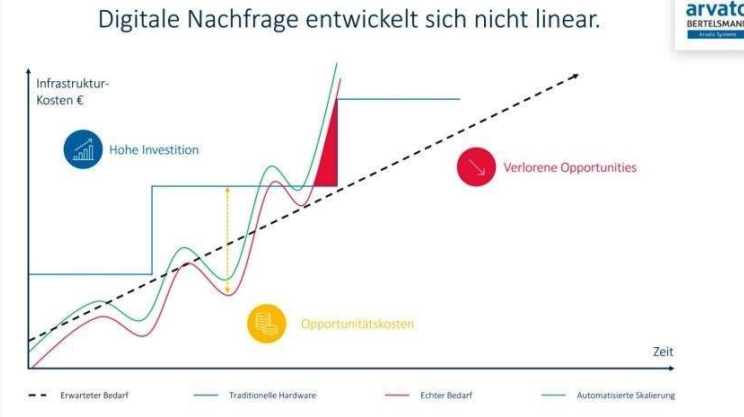
\includegraphics[width=\textwidth]{PreisEntwicklung.png}
    \caption{Entwicklung von Cloud- und On-Prem-Preisen}
\end{figure}
Bei On-Prem hat man hohe CapEx-Kosten, dies sind Investitionskosten. Durch die hohen Ausgaben hat man weniger Geld zur Verfügung und somit Opportunitätskosten, da man dieses Geld sonst in andere Dinge hätte investieren können. Bei der Cloud hat man hingegen OpEx-Kosten. Man gibt also immer wieder Geld aus, aber nicht viel auf einmal. Über die lange Zeit ist die Cloud von den Kosten her teurer, aber dafür hat man mehr Chancen, weil man nicht so viel vorab investieren musste.
       % CapEx/OpEx, Preismodelle, FinOps
\section{Cloud und Migration}
Unter Migration versteht man den Vorgang, bei dem ein bestehendes System -- etwa Daten, Anwendungen oder ganze IT-Infrastrukturen -- aus seiner bisherigen Umgebung in eine neue Zielumgebung überführt wird. Im Kontext der Cloud bedeutet das in der Regel, dass lokal betriebene Ressourcen (On-Premises) zu einem Cloud-Anbieter verlagert werden.

Ein anschauliches Beispiel: Bislang nutzt ein Unternehmen Office-Software wie Word und speichert seine Daten lokal, etwa auf einem On-Premises-NAS. Bei der Migration in die Cloud steigt man stattdessen auf Microsoft~365 um. Dadurch nutzt man nicht nur den Cloud-Storage von Microsoft, sondern erhält zusätzlich Dienste wie Teams oder Tools wie Power Automate und viele weitere M365-Features.

Man erkennt also: Eine Migration kann durchaus sinnvoll sein. Allerdings bringt sie auch einen nicht zu unterschätzenden Nachteil mit sich, nämlich die laufenden Kosten und die Bindung an Subscriptions (Abo-Modelle). Gerade bei M365 fallen fortlaufend Kosten an; durch Alternativen wie OpenOffice oder LibreOffice könnte man viel Geld sparen. Dafür bräuchte man jedoch einen eigenen Server mit Storage, hätte kein Teams und nur ein On-Premises Active Directory -- sofern man überhaupt Windows nutzt. Durch M365 erhält man dagegen ein Active Directory in der Cloud (Entra ID) und kann Benutzerrechte auch auf anderen Betriebssystemen durchsetzen.

\subsection{Use Cases für Cloud Migration}
Oben wurde nur ein einzelnes Beispiel genannt, was durch Cloud-Migration möglich ist. In realen Umgebungen gibt es jedoch mehrere wichtige Use Cases für eine Cloud-Migration. % LEKTORAT (fachlich): Überschrift sagte "6 R\,s", die Liste enthält jedoch
% sieben Punkte. Ursprünglich sind es sechs R\,s (Gartner/AWS); Relocate kam
% später als siebtes hinzu. Formulierung entsprechend angepasst.
Diese werden häufig als die \enquote{R\,s} der Migration zusammengefasst -- ursprünglich sechs (Rehost, Replatform, Repurchase, Refactor, Retire, Retain), häufig ergänzt um Relocate.

\subsubsection{Rehosting — Lift \& Shift}
Der Name Rehosting beziehungsweise Lift~\&~Shift oder auch As-is-Migration sagt bereits alles aus, was man wissen muss: Eine alte Anwendung wird mit minimalen Änderungen -- meist nur Anpassungen an den Umgebungsvariablen -- in der Cloud gehostet. Beispielsweise wird ein altes ERP-System vom eigenen Server genommen und in der Cloud in einer VM betrieben. Lift~\&~Shift sollte eigentlich keine dauerhafte Lösung sein, sondern eine Übergangslösung. Wer wirklich in die Cloud migrieren will, sollte keine monolithische Legacy-Anwendung weiterverwenden, sondern auf eine Microservice-Architektur setzen.

\subsubsection{Replatforming — Lift, Tinker \& Shift}
Replatforming ist im Grunde ein Lift~\&~Shift, bei dem man die Anwendung jedoch an die Cloud anpasst und dabei auch PaaS-Angebote nutzt -- beispielsweise eine Managed-PostgreSQL-Datenbank und Kubernetes (K8s). Man überführt also eine On-Premises-Anwendung mit gezielten Änderungen hin zu einer Cloud-nativen Anwendung, ohne sie jedoch komplett neu zu schreiben.

\subsubsection{Repurchasing}
Auch als \enquote{Drop and Shop} bekannt; das oben genannte Beispiel erklärt es recht gut. Man nutzt eine lizenzierte Software und kauft statt der On-Premises-Lizenzen eine Lizenz für das entsprechende Cloud-Angebot -- meist sogar beim selben Anbieter. Häufig wechselt man dabei von einem klassischen Lizenzkauf zu einem SaaS-Abo-Modell.

\subsubsection{Refactoring}
Refactoring ist wie Replatforming, nur noch deutlich umfangreicher: Man passt eine Anwendung vollständig an die Cloud an und baut eine monolithische Software in eine serviceorientierte Architektur (Microservices) um. Dieser Ansatz ist am aufwendigsten und teuersten, schöpft das Potenzial der Cloud (Skalierbarkeit, Elastizität) dafür aber am besten aus.

\subsubsection{Relocate}
Bei Relocate werden VM-Workloads in die Cloud verschoben, ohne die Anwendung selbst anzupassen. Im Unterschied zu Rehosting geschieht dies oft auf Infrastrukturebene, etwa durch das Verschieben ganzer VMware-Umgebungen, ohne jede Anwendung einzeln neu aufzusetzen.

\subsubsection{Retiring}
Eine Anwendung wird nicht mehr verwendet, verbraucht aber noch Ressourcen. Im Zuge der Migration wird sie identifiziert und abgeschaltet, was Kosten spart.

\subsubsection{Retaining}
Legacy-Apps, die vorerst nicht migriert werden -- etwa weil sich eine Migration (noch) nicht lohnt oder technische bzw. rechtliche Hürden bestehen. Sie verbleiben bewusst On-Premises.
    % Migration in die Cloud, 6 R's (Rehosting …)
\section{Cloud und Datenschutz}

\subsection{Data Sovereignty}
Regionale Datenschutzvorgaben verlangen, dass Daten physisch in
bestimmten Gebieten gespeichert werden. Cloud-Anbieter nutzen zwar
geografisch verteilte Replikation für hohe Verfügbarkeit, jedoch kann
diese verteilte Speicherung gegen lokale Vorschriften verstoßen.
Eine Daten-Souveränitäts-Architektur stellt sicher, dass geschützte
Daten regelkonform abgelegt werden. Replikationsmechanismen müssen
daher Compliance-fähig konfigurierbar sein, und Daten-Governance
koordiniert die Speicherung in den jeweils vorgeschriebenen Regionen.

\subsection{Sovereign Cloud}
Eine Sovereign Cloud schützt personenbezogene Daten, geistiges
Eigentum, Software und Finanzdaten unter staatlicher oder regionaler
Kontrolle. Sie besteht aus drei Souveränitätsebenen:
\begin{itemize}
    \item \textbf{Daten-Souveränität:} Schlüsselkontrolle und Speicherort
    \item \textbf{Betriebs-Souveränität:} Verfügbarkeit und Regionalität
    \item \textbf{Digitale Souveränität:} Zugriffs-Policies und Transparenz
\end{itemize}

Technisch wird das umgesetzt durch Verschlüsselung,
\textit{Keep-Your-Own-Key} und Confidential Computing.
Der Betrieb erfolgt entweder über öffentliche Cloud mit regionalen
Rechenzentren (z.\,B. Frankfurt) oder über Hybrid-Plattformen wie
OpenShift. Compliance wird durch \textit{Policy-as-Code} und
kontinuierliche Überwachung sichergestellt.\\[4pt]
\textbf{Risikobasierter Ansatz:} Strenge Regeln gelten nur für
kritische Workloads. Nicht-sensible Daten dürfen EU-weit fließen,
kritische Daten (Gesundheit, Behörden, Finanzen) müssen im jeweiligen
Land bleiben, nachweisbar.

\subsubsection{Warum Sovereign Cloud? – Rechtlicher Hintergrund}

\textbf{DSGVO (Datenschutz-Grundverordnung):}
Die DSGVO ist eine EU-Verordnung (seit 2018), die den Umgang mit
personenbezogenen Daten regelt. Sie gilt für alle Unternehmen, die
Daten von EU-Bürgern verarbeiten, unabhängig davon, wo das Unternehmen
selbst sitzt. Kernanforderungen sind Zweckbindung, Datensparsamkeit,
nachweisbare Einwilligung und das Recht auf Löschung. Ergänzt wird
sie in Deutschland durch das \textbf{BDSG} (Bundesdatenschutzgesetz).

\textbf{US CLOUD Act (Clarifying Lawful Overseas Use of Data Act):}
Ein US-amerikanisches Gesetz (seit 2018), das US-Behörden erlaubt,
von amerikanischen Cloud-Anbietern (z.\,B. AWS, Azure, Google Cloud)
Herausgabe von Daten zu verlangen, auch wenn diese Daten physisch
in der EU liegen. Das untergräbt den DSGVO-Schutz, denn selbst ein
deutsches Rechenzentrum von Microsoft unterliegt dem CLOUD Act,
solange Microsoft ein US-Unternehmen ist.

\textbf{FISA 702 (Foreign Intelligence Surveillance Act):}
Ermöglicht US-Geheimdiensten den Zugriff auf Kommunikationsdaten
ausländischer Personen, die über US-amerikanische Dienste laufen,
ohne richterliche Einzelgenehmigung.\\[4pt]
Die Sovereign Cloud soll genau diese Zugriffsmöglichkeiten
durch technische und organisatorische Maßnahmen verhindern,
zum Beispiel durch europäische Betreiber ohne US-Mutterkonzern
oder durch Verschlüsselung, bei der nur der Kunde den Schlüssel hält.

\subsection{Governance}
Governance beschreibt die Möglichkeit eines Unternehmens, Anwendungen unternehmensweit 
zu steuern, Compliance nachzuweisen und Risiken zu kontrollieren. Hierfür existieren 
vordefinierte Prinzipien, Gremien und Reviews. Governance besteht aus vier Domänen:
\begin{itemize}
    \item \textbf{Geschäftsarchitektur}
    \item \textbf{Anwendungsarchitektur}
    \item \textbf{Datenarchitektur}
    \item \textbf{Technologiearchitektur}
\end{itemize}

\subsection{Personenbezogene Daten}
Daten, die eine natürliche Person identifizieren oder identifizierbar machen, sind personenbezogene Daten. Besonders schützenswert (besondere Kategorien nach Art. 9 DSGVO) sind Rasse, Ethnie, politische Meinung, Religion, Weltanschauung, Gewerkschaftszugehörigkeit, sexuelle Identität, Gesundheit sowie genetische und biometrische Daten. Daten bei unter 16-Jährigen sind nur mit der Zustimmung der Eltern zu speichern. Personenbezogene Daten können anonymisiert werden.

\clearpage
\section{Glossar}

Kompaktes Nachschlagewerk der wichtigsten Begriffe aus diesem Lernzettel.
Jeder Eintrag ist bewusst kurz gehalten -- als Gedächtnisstütze für die Klausur,
nicht als Ersatz für die ausführlichen Kapitel.

% ── Formatierung der Begriffsliste ────────────────────────────────────────
% Begriff fett in Akzentfarbe, Erklärung im Fließtext dahinter.
\newlist{glossar}{description}{1}
\setlist[glossar]{
  style       = unboxed,
  leftmargin  = 0pt,
  itemsep     = 4pt,
  parsep      = 0pt,
  font        = {\normalfont\bfseries\color{primary}},
}

\begin{glossar}

  \item[Allocating] Zuweisung bereits bereitgestellter Ressourcen zu konkreten
        Workloads inkl.\ Kostenzuordnung (Tagging) auf Teams oder Projekte.

  \item[Availability (Hochverfügbarkeit)] Anteil der Zeit, in dem ein Dienst
        funktionsfähig ist, meist in „Neunen“ angegeben (z.\,B.\ 99,99\,\%);
        vertraglich im \emph{SLA} zugesichert.

  \item[Big Data] Verarbeitung sehr großer, schnell wachsender und vielfältiger
        Datenmengen, für die klassische Systeme nicht mehr ausreichen
        (Volume, Velocity, Variety).

  \item[Broad Network Access] NIST-Eigenschaft: Cloud-Dienste sind über das Netz
        standardisiert und geräteunabhängig (Laptop, Smartphone, \dots) erreichbar.

  \item[CapEx (Capital Expenditure)] Investitionsausgaben für eigene Hardware/
        Infrastruktur, die als Anlagevermögen über Jahre abgeschrieben wird.

  \item[CDN (Content Delivery Network)] Verteiltes Netz aus Edge-Servern, das
        Inhalte nahe beim Nutzer zwischenspeichert und so Latenz und Last senkt.

  \item[CI/CD] Continuous Integration / Continuous Delivery: automatisiertes
        Bauen, Testen und Ausliefern von Software in kurzen, häufigen Zyklen.

  \item[Cloud Auditor] Akteur (NIST), der Cloud-Dienste unabhängig auf Sicherheit,
        Datenschutz und Performance prüft.

  \item[Cloud Broker] Vermittler, der Cloud-Dienste mehrerer Provider bündelt,
        anpasst oder weiterverkauft.

  \item[Cloud Bursting] Hybrides Muster: Lastspitzen werden temporär aus der
        Private Cloud in die Public Cloud ausgelagert.

  \item[Cloud Carrier] Anbieter der Netzanbindung (Konnektivität), der Consumer
        und Provider verbindet -- typischerweise der \emph{ISP}.

  \item[Cloud Consumer] Nutzer bzw.\ Kunde, der Cloud-Dienste bezieht und verwendet.

  \item[Cloud Native] Entwurfsansatz für Anwendungen, die gezielt für die Cloud
        gebaut sind: Microservices, Container, Automatisierung, Elastizität.

  \item[Cloud Provider] Anbieter, der Cloud-Ressourcen und -Dienste bereitstellt
        und betreibt (z.\,B.\ AWS, Azure, GCP).

  \item[Cluster] Verbund mehrerer Rechner (Nodes), die zusammenarbeiten und
        nach außen wie ein System wirken (Ausfallsicherheit, Lastverteilung).

  \item[Compute] Rechenleistung der Cloud (CPU/RAM) -- bereitgestellt als VMs,
        Container oder Functions.

  \item[Container] Leichtgewichtige, isolierte Laufzeitumgebung, die eine
        Anwendung mit allen Abhängigkeiten kapselt; teilt sich den Kernel des Hosts.

  \item[Container Registry] Zentraler Speicher für Container-Images (z.\,B.\
        Docker Hub), aus dem Images verteilt und abgerufen werden.

  \item[Data Sovereignty (Datensouveränität)] Grundsatz, dass Daten den Gesetzen
        des Landes unterliegen, in dem sie gespeichert/verarbeitet werden.

  \item[DevOps] Kultur und Praxis, die Entwicklung (Dev) und Betrieb (Ops) eng
        verzahnt -- mit Automatisierung, CI/CD und gemeinsamer Verantwortung.

  \item[Disaster Recovery] Wiederherstellung von Systemen und Daten nach einem
        Ausfall/Katastrophenfall (gemessen über RTO und RPO).

  \item[Docker] Verbreitete Plattform zum Bauen, Verteilen und Ausführen von
        Containern auf Basis von Images.

  \item[Egress] Ausgehender Datenverkehr aus der Cloud heraus -- bei Providern
        häufig kostenpflichtig (vgl.\ \emph{Ingress}).

  \item[Elastizität (Elasticity)] Automatisches, schnelles Hoch- und
        Herunterskalieren von Ressourcen entlang der tatsächlichen Last.

  \item[FaaS (Function as a Service)] Serverless-Modell, bei dem einzelne
        Funktionen ereignisgesteuert ausgeführt und sekundengenau abgerechnet werden.

  \item[FinOps] Disziplin zur Steuerung und Optimierung von Cloud-Kosten als
        gemeinsame Verantwortung von Technik, Finanzen und Business.

  \item[Governance] Regeln, Rollen und Kontrollen, die Cloud-Nutzung steuern
        (Sicherheit, Compliance, Kosten, Standards).

  \item[Horizontale Skalierung] Leistung erhöhen durch \emph{mehr} Instanzen
        (Scale-out) statt durch stärkere einzelne Maschinen.

  \item[Hybrid Cloud] Kombination aus Private und Public Cloud, die als Verbund
        zusammenarbeiten (ermöglicht z.\,B.\ Cloud Bursting).

  \item[Hypervisor] Software-Schicht, die physische Hardware in mehrere
        virtuelle Maschinen aufteilt und verwaltet (Typ\,1: bare-metal, Typ\,2: hosted).

  \item[Hyperscaler] Sehr großer Cloud-Anbieter mit global verteilten
        Rechenzentren und enormer Skalierung (AWS, Microsoft Azure, Google Cloud).

  \item[IaaS (Infrastructure as a Service)] Bereitstellung virtualisierter
        Infrastruktur (Rechenleistung, Speicher, Netz); Kunde verwaltet OS und Anwendung.

  \item[Image] Unveränderliche Vorlage, aus der Container (oder VMs) gestartet
        werden -- enthält Anwendung samt Abhängigkeiten.

  \item[Ingress] Eingehender Datenverkehr in die Cloud hinein; meist kostenlos.
        In Kubernetes zugleich die Regelschicht für externen Zugriff auf Services.

  \item[Instanz] Konkrete, laufende Ausprägung einer Ressource, z.\,B.\ eine
        gestartete virtuelle Maschine.

  \item[ISP (Internet Service Provider)] Anbieter des Internetzugangs; stellt die
        Netzanbindung bereit und übernimmt damit die Rolle des \emph{Cloud Carrier}.

  \item[Kubernetes] Orchestrierungsplattform, die containerisierte Anwendungen
        automatisch verteilt, skaliert, überwacht und neu startet.

  \item[Leaf-Spine-Architektur] Modernes, flaches Rechenzentrums-Netz, in dem
        jeder Leaf-Switch mit jedem Spine-Switch verbunden ist (gut für Ost-West-Verkehr).

  \item[Load Balancer] Komponente, die eingehende Anfragen auf mehrere Instanzen
        verteilt -- für Lastausgleich und Ausfallsicherheit.

  \item[Measured Service] NIST-Eigenschaft: Ressourcennutzung wird gemessen,
        überwacht und transparent abgerechnet (Grundlage für \emph{Pay per Use}).

  \item[Microservices] Architektur aus vielen kleinen, unabhängig
        deploybaren Diensten statt einer großen Anwendung (vgl.\ \emph{Monolith}).

  \item[Monolith] Anwendung, bei der alle Funktionen in einer einzigen,
        eng gekoppelten Codebasis stecken und gemeinsam ausgeliefert werden.

  \item[NIST] National Institute of Standards and Technology; liefert die
        anerkannte formale Definition von Cloud Computing (5 Eigenschaften).

  \item[Node] Einzelner Rechner (physisch oder virtuell) innerhalb eines Clusters,
        in Kubernetes Träger der Pods.

  \item[On-Demand Self-Service] NIST-Eigenschaft: Nutzer beziehen Ressourcen
        selbstständig und automatisiert, ohne menschliches Zutun des Providers.

  \item[OpEx (Operational Expenditure)] Laufende Betriebskosten (z.\,B.\
        nutzungsbasierte Cloud-Gebühren) statt einmaliger Investition -- vgl.\ \emph{CapEx}.

  \item[Ost-West-Verkehr] Datenverkehr \emph{zwischen} Servern innerhalb des
        Rechenzentrums; Nord-Süd-Verkehr verläuft von außen nach innen und umgekehrt.

  \item[PaaS (Platform as a Service)] Bereitstellung einer fertigen
        Entwicklungs-/Laufzeitplattform; Kunde kümmert sich nur um Code und Daten.

  \item[Pay per Use] Abrechnung nach tatsächlicher Nutzung statt fester
        Pauschale -- ermöglicht durch \emph{Measured Service}.

  \item[Personenbezogene Daten] Informationen, die sich auf eine identifizierte
        oder identifizierbare natürliche Person beziehen (Kernbegriff der DSGVO).

  \item[Pod] Kleinste deploybare Einheit in Kubernetes; enthält einen oder
        mehrere eng zusammengehörige Container.

  \item[Private Cloud] Cloud-Infrastruktur, die exklusiv für eine einzelne
        Organisation betrieben wird (mehr Kontrolle, höhere Eigenverantwortung).

  \item[Provisioning] Dynamische Bereitstellung von Ressourcen, sobald sie
        angefordert werden.

  \item[Public Cloud] Über das Internet öffentlich angebotene, geteilte
        Cloud-Infrastruktur eines Providers (Mehrmandantenfähigkeit).

  \item[Rapid Elasticity] NIST-Eigenschaft: Ressourcen lassen sich sehr schnell,
        scheinbar unbegrenzt, automatisch erweitern und reduzieren.

  \item[Rechenzentrum] Gebäude/Einrichtung mit Servern, Netz, Strom- und
        Kühlinfrastruktur, in der Cloud-Ressourcen physisch betrieben werden.

  \item[Refactoring] Migrations-R: Anwendung wird umgebaut/neu strukturiert,
        um Cloud-Vorteile (z.\,B.\ Cloud Native) voll zu nutzen.

  \item[Region] Geografisches Gebiet eines Providers, das mehrere
        \emph{Verfügbarkeitszonen} bündelt.

  \item[Rehosting (Lift \& Shift)] Migrations-R: Anwendung wird unverändert
        in die Cloud verschoben -- schnell, aber ohne Cloud-Optimierung.

  \item[Replatforming (Lift, Tinker \& Shift)] Migrations-R: kleine Anpassungen
        bei der Migration, ohne die Kernarchitektur zu ändern.

  \item[Repurchasing] Migrations-R: Wechsel auf ein anderes (meist SaaS-)Produkt
        statt der bisherigen Anwendung.

  \item[Reservierung (Reserved Instances)] Vorab-Buchung von Kapazität über
        längere Laufzeit gegen deutlichen Rabatt gegenüber On-Demand.

  \item[Resource Pooling] NIST-Eigenschaft: Ressourcen werden gebündelt und
        mehreren Kunden mandantenfähig zugeteilt (ermöglicht durch Virtualisierung).

  \item[Retaining] Migrations-R: Anwendung bleibt bewusst dort, wo sie ist
        (kein Umzug, z.\,B.\ wegen Aufwand oder Vorgaben).

  \item[Retiring] Migrations-R: nicht mehr benötigte Anwendungen werden
        abgeschaltet.

  \item[SaaS (Software as a Service)] Fertige Anwendung als Dienst über das Netz;
        Provider verantwortet die komplette Infrastruktur (z.\,B.\ Microsoft~365).

  \item[Savings Plans] Rabattmodell mit Verpflichtung zu einer bestimmten
        Nutzung/Ausgabe pro Stunde über eine Laufzeit.

  \item[Serverless] Modell, bei dem der Provider die Server vollständig
        verwaltet; der Nutzer denkt nur in Funktionen/Diensten (vgl.\ \emph{FaaS}).

  \item[Service Discovery] Mechanismus, mit dem Dienste sich gegenseitig
        automatisch finden und adressieren (wichtig bei Microservices).

  \item[Shared Responsibility Model] Aufteilung der Sicherheitsverantwortung
        zwischen Provider und Kunde -- je nach Servicemodell (IaaS/PaaS/SaaS) verschieden.

  \item[Skalierung (Scalability)] Fähigkeit eines Systems, mit wachsender Last
        durch zusätzliche Ressourcen mitzuwachsen (horizontal oder vertikal).

  \item[SLA (Service Level Agreement)] Vertrag, der zugesicherte Dienstgüte
        (z.\,B.\ Verfügbarkeit) und Folgen bei Nichteinhaltung festlegt.

  \item[Sovereign Cloud] Cloud, die durch Standort und Betrieb die Einhaltung
        nationaler/europäischer Rechts- und Datenschutzvorgaben garantiert.

  \item[Spot Instances] Sehr günstige, ungenutzte Cloud-Kapazität, die der
        Provider jederzeit kurzfristig zurückfordern kann.

  \item[Technische Schulden] Spätere Mehrkosten durch heute bewusst oder
        unbewusst gewählte schnelle, aber suboptimale Lösungen.

  \item[3-Tier-Architektur] Klassisches Schichtmodell aus Präsentations-,
        Logik- und Datenschicht (im Netz auch als Access/Aggregation/Core).

  \item[TOGAF] Verbreitetes Enterprise-Architektur-Framework mit der
        Architecture Development Method (ADM) als Vorgehensmodell.

  \item[Verfügbarkeitszone (Availability Zone)] Eigenständiges Rechenzentrum
        (oder Gruppe) innerhalb einer Region, gegen Ausfälle voneinander isoliert.

  \item[Vertikale Skalierung] Leistung erhöhen durch \emph{stärkere} Hardware
        einer Instanz (Scale-up) statt durch zusätzliche Instanzen.

  \item[Virtualisierung] Abstraktion physischer Hardware in mehrere virtuelle
        Einheiten -- technische Grundlage für Resource Pooling und Cloud.

  \item[Virtuelle Maschine (VM)] Software-Nachbildung eines vollständigen
        Rechners samt eigenem Betriebssystem, vom Hypervisor bereitgestellt.

  \item[VPC (Virtual Private Cloud)] Logisch isoliertes, privates Netz innerhalb
        der Public Cloud, in dem eigene Ressourcen abgesichert betrieben werden.

  \item[Zero Downtime] Bereitstellung von Updates ohne spürbare Ausfallzeit
        für die Nutzer (z.\,B.\ über Rolling Updates).

\end{glossar}

% ── Literaturverzeichnis ──────────────────────────────────────────────────


\end{document}
